\documentclass[12pt,a4paper,left=2cm,right=2cm,oneside,titlepage]{report}
\usepackage[xutf8]{inputenc}
\usepackage{amsmath}
\usepackage{amsfonts}
\usepackage{amssymb}
\usepackage{cases}
\numberwithin{equation}{section}
\usepackage{mathtools}
\usepackage{commath}
\usepackage{makeidx}
\usepackage{graphicx}
\usepackage{fancyhdr}
\usepackage[titletoc]{appendix}
\usepackage{listings}
\usepackage{color}
\definecolor{dkgreen}{rgb}{0,0.6,0}
\definecolor{gray}{rgb}{0.5,0.5,0.5}
\definecolor{mauve}{rgb}{0.58,0,0.82}

\lstset{frame=tb,
	language=R,
	aboveskip=3mm,
	belowskip=3mm,
	showstringspaces=false,
	columns=flexible,
	basicstyle={\small\ttfamily},
	numbers=none,
	numberstyle=\tiny\color{gray},
	keywordstyle=\color{blue},
	commentstyle=\color{dkgreen},
	stringstyle=\color{mauve},
	breaklines=true,
	breakatwhitespace=true,
	tabsize=3
}
\usepackage[unicode]{hyperref}
\setlength{\parskip}{1em}
\usepackage[top=3.5cm,bottom=3.5cm,left=2.5cm,right=2.5cm]{geometry}
\allowdisplaybreaks

\begin{document}
\thispagestyle{empty}

\begin{center}
	\fontsize{12pt}{18pt}\selectfont \textbf{VIETNAM NATIONAL UNIVERSITY – HO CHI MINH CITY\\
	INTERNATIONAL UNVERSITY\\
	DEPARTMENT OF MATHEMATICS} \vspace{0.8cm}
	
		\begin{figure}[htp]
			\begin{center}
				
\includegraphics[scale=.6]{logo}
			\end{center}
		\end{figure}	
	\begin{center}
		\fontsize{12pt}{18pt}\selectfont \textbf{GRADUATION THESIS:} \\ \vspace{36pt}
		
		\fontsize{14pt}{16pt}\selectfont \textbf{PRICING EUROPEAN BARRIER OPTIONS WITH REBATES} \\ \vspace{2pt}
		
		\fontsize{12pt}{18pt}\selectfont \textbf{Submitted in partial fulfillment of the requirements for the degree of \\
		BACHELOR OF ENGINEERING in\\ 
		FINANCIAL ENGINEERING AND RISK MANAGEMENT} \\ \vspace{18pt}
		
			\fontsize{12pt}{18pt}\selectfont \textbf{Student’s Name:	Ta Thi Phuong Dung\\
		Student’s ID:	MAMAIU13067\\
		Thesis Supervisor:	Dr. Le Nhat Tan}
		
	\end{center}
\end{center}

\vspace{4.4cm}

\begin{center}
	\fontsize{12pt}{18pt}\selectfont \textbf{Ho Chi Minh City, Vietnam \\
    January, 2018}
\end{center}

\newpage
\pagenumbering{roman}
\begin{center}
	\fontsize{12pt}{18pt}\selectfont \textbf{VIETNAM NATIONAL UNIVERSITY – HO CHI MINH CITY\\
		INTERNATIONAL UNVERSITY} \vspace{0.8cm}
	
	\begin{figure}[htp]
		\begin{center}
			
\includegraphics[scale=.6]{logo}
		\end{center}
		\label{reflogo}
	\end{figure}	
	\begin{center}
		\fontsize{12pt}{18pt}\selectfont \textbf{GRADUATION THESIS:} \\ \vspace{36pt}
		
		\fontsize{14pt}{16pt}\selectfont \textbf{PRICING EUROPEAN BARRIER OPTIONS WITH REBATES} \\ \vspace{2pt}
		
		\fontsize{12pt}{18pt}\selectfont \textbf{Submitted to DEPARTMENT OF MATHEMATICS \\
			In partial fulfillment of the requirements for the degree of \\
			BACHELOR OF ENGINEERING in\\ 
			FINANCIAL ENGINEERING AND RISK MANAGEMENT} \\ \vspace{18pt}
		
		\fontsize{12pt}{18pt}\selectfont \textbf{Student’s Name:	Ta Thi Phuong Dung\\
			Student’s ID:	MAMAIU13067\\
			Thesis Supervisor:	Dr. Le Nhat Tan}
		
	\end{center}
\end{center}

\vspace{4.4cm}

\begin{center}
	\fontsize{12pt}{18pt}\selectfont \textbf{Ho Chi Minh City, Vietnam\\
	January, 2018}
\end{center}

\newpage

\begin{center}
	\fontsize{11pt}{18pt}\selectfont \textbf{PRICING EUROPEAN BARRIER OPTIONS WITH REBATES}\\
	\fontsize{11pt}{18pt}\selectfont By\\
	TA THI PHUONG DUNG\\ \vspace{18pt}

	SUBMITTED TO DEPARTMENT OF MATHEMATICS,\\
	INTERNATIONAL UNIVERSITY, HO CHI MINH CITY\\
	IN PARTIAL FULFILLMENT OF REQUIREMENTS FOR THE DEGREE OF\\ BACHELOR OF ENGINEERING IN FINANCIAL ENGINEERING AND RISK MANAGEMENT\\
	JANUARY 2018 	
\end{center}

	\vspace{54pt}	
\fontsize{12pt}{0pt}\selectfont Signature of Student: \hspace{50pt}\rule[0.02cm]{8cm}{0.0006cm} \\
\begin{flushright}
	Ta Thi Phuong Dung
\end{flushright} \vspace{18pt}
\hspace{14pt} \fontsize{12pt}{0pt}\selectfont Certified by: \hspace{94pt}\rule[0.02cm]{8cm}{0.0006cm} \\
\begin{flushright}
	Le Nhat Tan, Dr.\\ \vspace{10pt}
	Thesis Supervisor
\end{flushright}  \vspace{18pt}
\hspace{14pt} \fontsize{12pt}{0pt}\selectfont Approved by: \hspace{90pt}\rule[0.02cm]{8cm}{0.0006cm} \\
\begin{flushright}
	Assoc. Prof. Pham Huu Anh Ngoc\\ \vspace{10pt}
	Head of Department of Mathematics
\end{flushright}

\chapter*{Acknowledgements}

\addcontentsline{toc}{chapter}{Acknowledgements}
\fontsize{11pt}{20pt}\selectfont  First of all, I would like to express my very great appreciation to Dr. Le Nhat Tan for his valuable and constructive suggestions during the planning and development on my research work. His willingness to give his time so generously has been very much appreciated. He has given me practical and urgent research topics for my choice. Moreover, whatever topic I chose, he always supports thoughtful reference materials related to that topic. More meaningful things, are his extensive knowledge of financial mathematics and dedication to education, have given me a passion and a great source of knowledge about my subject. One of the things,  I really be grateful to him thanks to asking for troubles I was stuck in and reminding me to finish my thesis on time. Further, in order to get a good research, the thesis needs to gain not only right content, but also a logical and coherent structure which he taught me. \\[0.5cm]
Subsequently, I would also like to extend my thanks to all the lecturers at Department of Mathematics
(International University, IU-VNU), especially Assoc. Prof. Dr. Sc. Nguyen
Dinh, Assoc. Prof. Dr. Pham Huu Anh Ngoc, Assoc. Prof. Dr. Nguyen Ngoc Hai, Dr. Nguyen Minh Quan. Under their endless efforts and excellent teaching, I have received a useful mathematical knowledge along with some practical experiences supporting my future work. Especially, I have the foundation of mathematics to solve problems about financial mathematics in this research. \\[0.5cm]
Last but not least, my special thanks should be given to my family for their loving
support, motivation and patience during the undergraduate years. I wish to thank my university friends, especially Do Duy Viet and Ha Thi Phi Yen for making me happy to go to school and being interested in learning.\\[0.5cm] 
 One can say that I am very fortunate to have a good learning environment as International University, a dedicated advisor, and a great family, all things I cannot gain today without them. Again thank all of you from my heart.

 
  \chapter*{Abstract}
  
 \addcontentsline {toc}{chapter}{ Abstract} 
\fontsize{11pt}{20pt}\selectfont  In Vietnam, derivatives market has just started officially very recently, in August, 2017, with futures contracts on VN30 index. It is a very new investment area for Vietnamese investors. This market is however expected to strongly develop soon and then enhance greatly Vietnamese economy. In fact, trading volume on futures contracts on VN30 index is increasing significantly over last few months, and is expected to increase with an even faster rate. One important type of financial derivatives products is options. In Vietnam, covered call (a type of call options) will be traded soon. Options will bring greater leverage to speculators and bring more risk management tools for hedgers. Options thus have great potential chance in Vietnamese financial markets. Understanding clearly the pricing formulas for these products is very urgent, then the object of the thesis formulate the pricing models of European barrier options with rebates using the probabilistic approach. It includes deriving the Black - Scholes - Merton model by the Martingale approach which is model of European options. Then European down and out call options with rebates is formulated by using theory of Wiener process like Reflection Principle, First Passage Time, Markov Property and Stochastic Differential Equations as It\=o Calculus and One-Dimensional Diffusion Process. Further, testing real data for normal distribution using R – Studio software. Lastly, using the final formula to calculate the option price of the underlying asset price of stocks in Vietnam. The stock is applied that must be satisfied given conditions by previous testing. 

	\tableofcontents
	\listoffigures
	\listoftables
	
	\clearpage
	\chapter*{List of Abbreviations}
	
	RV \hspace{1cm} Random Variable\\[0.2cm]
	PDF \hspace{0.7cm} Probability Density Function\\[0.2cm]
	CDF \hspace{0.7cm} Cumulative Density Function\\[0.2cm]
	SDE \hspace{0.7cm} Stochastic Differential Equation\\[0.2cm]
	PDE \hspace{0.7cm} Partial Differential Equation\\[0.2cm]
	GBM \hspace{0.6cm} Geometric Brownian Motion\\[0.2cm]
	LN \hspace{1cm} Log-Normal
	 
	
	
	\newpage
	\pagenumbering{arabic}
	\setcounter{page}{1}	
	\chapter{Introduction}
\label{ch:Introduction}

	In the financial markets around the world, derivative instruments can be derived from Sixth Century B.C. Renowned philosopher of Greece; Thalus is thought to be the first person that had formulated a deal, which is alike to that of option derivative of today, for making profit.
A derivative is a security with a price that is dependent upon or derived from one or more underlying assets.
The derivative itself is a contract between two or more parties based upon the asset or assets.
 Value of a derivative changes with price change of its underlying asset (share, commodity, currency and many more). With the passage of time, the need of these instruments increased among various sections of the society for hedging purposes. Later, the speculative motive of the investors also surfaced and led to its popularity.\\[0.5cm]
Considering the given situation, pricing options is very important for the financial markets. In order to solve that issue, the use of mathematical techniques is a force of thing for formulating of the pricing of the option contracts. Mathematical models have been used in economics for a long time. By now, operations research, econometrics and time series analysis constitute major parts of curricula of business schools and economics departments.
Therefore, we will go into the complexity of the financial market to see how it needs some our  mathematical techniques .

\section{The structure of the financial market }
\fontsize{11pt}{20pt}\selectfont In the financial markets of economic system, we have found out two different sectors. They are household who saves money and business who needs money for the purpose of prodution or sale of goods and services. Financial market acts as an intermediary between the savers and investors of money where traders buy and sell stocks, bonds, derivatives, foreign exchange and commodies.\\[0.5cm]
There are three conditions to classifying market. Firstly, based on working capital, we have primary market where the new security issues sold to initial buyers. Typically involves an investment bank who underwrites the offering and second market where Securities previously issued are bought and sold. Involves both brokers and dealers. Secondly, based on operating approach, markets be assigned by exchange market that Stock trades conducted via centralized place. Buy/sell is conducted through the exchange; no direct contract between seller and buyer and OTC market (Over-The-Counter) where no centralized place. Trading is done directly between two parties, without the supervision of an exchange. Lastly, based on goods, there are stock market, bond market and derivative instrument. Let's look at stock market, a financial market that enables investors to buy and sell shares of publicly traded companies. There are common stock and preferred stock. Then bond market, a financial market where participants can issue new debt  or buy and sell debt securities. The form may be bonds, notes, bills, and so on. For derivative instrument, a financial market that trades securities that derive its value from its underlying asset including stock right, warrant, option. In this research, options will be analized for deriving the formula.  
\section{Options}
Options are a type of derivative security. They are a derivative because the price of an option is intrinsically linked to the price of something else. Specifically, options are contracts that grant the right, but not the obligation to buy or sell an underlying asset at a set price on or before a expiration date. The right to buy is called a call option and the right to sell is a put option. A call option, might be thought of as a deposit for a future purpose, is bought if the trader expects the price of the underlying to rise within a certain time frame. For example, let's say you purchase a call option on shares of Intel (INTC) with a strike price which is a fixed at which an asset may be bought or sold of $\$40$ and an expiration date of May 16th. This option would give you the right to purchase 100 shares of Intel at a price of $\$40$ on May 16th (the right to do this, of course, will only be valuable if Intel is trading above $\$40$ per share at that point in time) and you will pay option premium for the writer. Conversely, a put option is bought if the trader expects the price of the underlying to fall within a certain time frame.  \\[0.5cm]
At a premium, since the writer of an option is exposed to potential liabilities in the future, he must be compensated with an up-front premium paid by the holder who has bought this option when they together enter into the option contract.  When you buy an option, the purchase price is called the premium. If you sell, the premium is the amount you receive. The premium isn't fixed and changes constantly. The premium is likely to be higher or lower today than yesterday or tomorrow. Changing prices reflect the give and take between what buyers are willing to pay and what sellers are willing to accept for the option. The point of agreement becomes the price for that transaction. \\ [0.5cm]
In addition, options can be categorized based on the method in which they are traded, their expiration cycle, and the underlying security they relate to. It is listed of some different common types of option: Barrier,
American, European, Asian, Lookback... This research will be focus into the combination of European and Barrier option that is more attractive and cheaper than the respective standard European options. 
	\subsection{European option}
	European options are contracts that give the holder the right but not the obligation, to buy or sell the underlying security at a specific price (the strike price) only on the option's expiration date. As the exercise date is limited in the European option, it removes the uncertainty about possible early execution. The lack of this uncertainty is expected to encourage more investors to trade stock options. Theoretically, a European option has lower value than an otherwise, it is because a European option does not enjoy the convenience that arises from flexibility in timing of exercise, which is a premium option. The holder must pay a premium at the initial time. This option is the path independent option. \\ [0.5cm]
	The path independent option whose payoff depends solely on the events specified to take place upon expiration, rather than the path taken by the underlying variable (price, rate, index, etc). An example for European option, if an investor buys a call option with a strike price of $\$20$, he would benefit if the underlying rises above $\$20$ upon expiration. If not, he would not exercise and the premium paid to buy the option is lost. We consider the payoffs for a European option that is value at the expiration time, as a function of the underlying stock price	
	\begin{center}
Call option = $\max(S-K,0)$\\
Put option = $\max(K-S,0)$\\
	\end{center}
Where\\
$S$: the current price\\
$K$: the strike price   \\[0.5cm]
Let's look at the following diagram which discribes profit of call option. Suppose that we have one call option with exercise price $\$50$ which costs $\$5$, the stock price moves from $\$0$ to $\$100$.  
\begin{figure}[htp]
	\begin{center}
		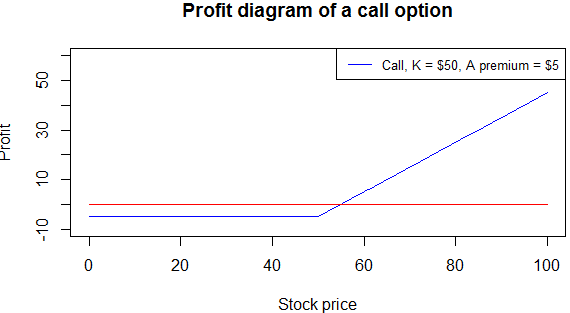
\includegraphics[scale=0.8]{Rplot02}
	\end{center}
	\label{refRplot02}
	\caption{Profit of a call option}
\end{figure}

The above diagram implies that if the stock price belows the strike price, the holder would not exercise the option and had to pay a premium of $\$5$. Conversely, if the stock price is higher than the strike price and differences between two of them is greater than zero, he would practice the option and receive profit which is equal to the stock price minus the strike price and a premium. 
	
	\subsection{Barrier option}
	The barrier option is the simpiest popular path dependent option. It is a type of option and its distinctive feature is that the payoff depends not
	only on the final price of the underlying asset, but also on whether the asset price has
	breached some barrier level during the life of the option. So, a barrier option’s payoff depends on two price levels:
	the strike price and the so-called barrier price. One of the important things is that the holder of the option may be compensated
	by a rebate payment for the cancellation of the option, that helps to keep losing all premium he paid before. Let's consider two most common types of barrier options are knock-out and knock-in barrier options. 	
	\begin{itemize}
		\item Knock-out barrier options is a type of barrier option becomes worthless if the underlying asset price touches the barrier. Moreover, it is also devided into two parts, down and out barrier option which implies if the underlying asset's price falls below the barrier at any point in the option's life, the option will be worthless and up and out barrier option which implies if the underlying asset’s price increases above the barrier at any point in the option’s life, the option will be worthless.
			
	\item Knock-in option has no value until the underlying asset price crosses the in-barrier. This option is classified as down and in barrier option which means if the underlying asset price moves below a barrier at any point in the option’s life, the option comes into existence and up and in barrier option which indicates if the price of the underlying asset rises above the barrier at any point in the option’s life, the option comes into existence.	
	\end{itemize}
Barrier options carry a higher risk to the holder than the more standard types of contracts. With a knock out contract,  the holder carries the risk of their investment basically ceasing to exist if the underlying security moves significantly and reaches the knock out price. With a knock in contract, if the underlying security only moves a little in price there may be no profits to be taken. There is, however, one significant advantage that barrier options offer traders, barrier options are generally cheaper than contracts that do not include a barrier price  because of the increased risk that the holder has to take.  The barrier options are popular and attractive thanks to benefits that they give investors more flexibility to express their view on the asset price movement in the option contract. The buyer can achieve {\itshape option premium reduction} through the barrier provision by not paying a premium to cover scenarios he or she views as unlikely. The option writer can limit liabilities when the asset price rises acutely. 
	\subsection{European barrier call option}
	It is a type of option including characters of both European option and barrier option which means the option will be exercised at expiration date unless the underlying asset price reached or exceeded a lower barrier during the option's life. Especially, the option cannot be activated again if the underlying asset price go up after down to a lower barrier. The distinctive features of call options and put options are just conversely like one is the right to buy the asset and hence benefit would be gained as the price of the underlying goes up and one is the right to sell the asset and hence benefit would be gained as the price of the underlying goes down. Therefore, we will focus on only one side and the call option will be analyzed.\\
		\begin{figure}[htp]
		\begin{center}
			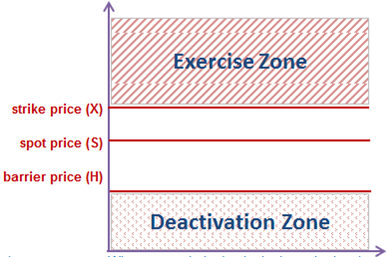
\includegraphics[scale=0.9]{figure1}
		\caption{Down and Out Call option $X > H$}
		\label{reffig1} 
	    \end{center}
     	\end{figure} \\
    Let's look at Figure ~\ref{reffig1}  which decribes Down and Out Call option when the strike price $(X)$ is greater than the barrier $(H)$. Expectation of the price will go up over the strike price to exercise option and make payoff is equal difference between the stock price at expiration date and the strike price. If the price goes down, the option will be deactivated.   
	\subsection{European barrier call option with rebates}
	This is a specified of European barrier call option which a knock-out occurs, the holder of the option will receive a partial rebate on the premium paid to the option writer. European barrier call option with rebates are cheaper than the respective standard European options because a zero payoff maybe occur before expiry time T. Lower premiums are usually offered for more exotic barrier option, which make them particularly attractive to hedgers in the financial market.\\[0.5cm]
	Let's illustrate this type of option by an example. We consider the European down-and-out call option under the underlying asset of XYZ stock, the current price is approximately, $\$39$ and rebate is $\$5$. If the XYZ price falls to $\$28$ which is a barrier level within the next six months. the writer will have to  pay $\$5$ dollars for the holder if XYZ stock is less than or equal to $\$28$ at any point in the next six months.
	\chapter{The Mathematical Background}
\label{ch:MB}

\section{Probability theory}

Probability theory is a part of mathematics that deals with mathematical models of trials
whose outcomes depend on chance. For the perspective of mathematical finance, we will go through
some basic concepts of probability theory that are needed to begin solving stochastic calculus
problems. It is not completed the whole prospect, but be sufficient for this research. %In particular, pricing the Black-Schole-Merton model and European barrier call option with rebates.
%We consider an experiment or a trial whose outcome is not predictable with certainty.
%The set of all possible outcomes of an experiment is called the sample space and we denote it
%by $\Omega$. Any subset A of the sample space is known as an event, where an event is a set consisting
%of possible outcomes of the experiment.
%The collection of events can be defined as a subcollection $\mathcal{F}$ of the set of all subsets of $\Omega$
%and we define any collection $\mathcal{F}$ of subsets of $\Omega$. \\


\subsection{Continuous Random Variables}
A continuous random variable is a random variable where the data can take infinitely many values. For example, heights of people in a population. Let's X is a continuous random variable, the cumulative distribution $F$ of $X$ is given by
\begin{align*}
	F(x) = P\{X\leq x\}
\end{align*}
We shall assume that there is some function f such that
\begin{align*}
		F(x) = \displaystyle \int_{-\infty}^{x}f(t)dt
\end{align*}
for all real number $x$, $f$ is known as the PDF for X. The PDF $f$ of a continuous random variable X satifies
\begin{enumerate}
	\item $f(x) \geq 0$ for all $x$;
	\item $\int_{-\infty}^{\infty}f(x)dx = 1$
	\item $P(a\leq X \leq b)=\int_{a}^{b}f(x)dx$ for all $a, b$.
\end{enumerate}
\begin{figure}[htp]
	\begin{center}
		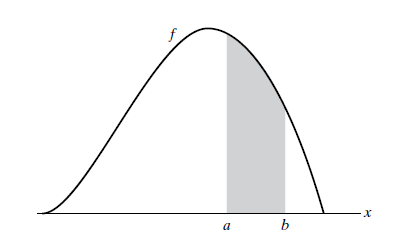
\includegraphics[scale=0.8]{figure6}
	\end{center}
	\label{reffig6}
	\caption{$P(a\leq X \leq b)$ = area of shaded region. }
\end{figure}
Probabilities correspond to areas under the curve $f(x)$. For any single value a, $P(X=a)=0$.\\
$P(a< X < b)=P(a\leq X < b)=P(a< X \leq b)=P(a\leq X \leq b)$.\\
The expected value of $X$,
\begin{align*}
	E[X] = \displaystyle \int_{-\infty}^{\infty}xf(x)dx
\end{align*}
The expected value of any real-valued function g,
\begin{center}
	$E[g(x)] = \displaystyle \int_{-\infty}^{\infty}g(x)f(x)dx$
\end{center}
The variance
\begin{align*}
	Var(X) = E[(X - \mu)^2] &= E[X^2]-(E[X])^2\\
	Var(aX+b) &= a^2\sqrt{Var(X)}
\end{align*}
Where\\
 $\mu$ : expected value of X\\
 $a, b$: real value
 
 \newpage
\subsection{Normal Random Variables}
	\begin{figure}[htp]
	\begin{center}
		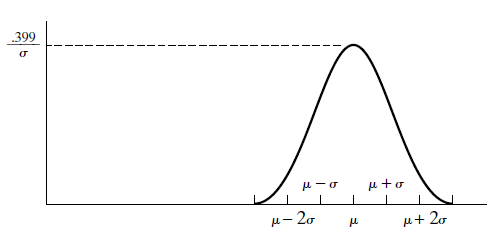
\includegraphics[scale=0.8]{figure3}
	\end{center}
	\label{reffig3}
	\caption{Arbitrary $\mu$, $\sigma^2$}
\end{figure}
X is a normal random variable (normally distributed) with parameter $\mu$ and $\sigma^2$, the density of X is given by
\begin{center}
	$f(x)=\dfrac{1}{\sqrt{2\pi}\sigma}e^\frac{-(x-\mu)^2}{2\sigma^2}  \hspace{3cm} -\infty\hspace{0.2cm}<\hspace{0.2cm} x\hspace{0.2cm}<\hspace{0.2cm}\infty$
\end{center}
If $Y=aX+b$, then $Y$ is normally distributed with parameter $a\mu+b$ and $a^2\sigma^2$.
\begin{itemize}
	\item The cumulative distribution of $Y$
	\begin{center}
		$F_Y(x)=P\{Y\leq x\}=F_X\left(\dfrac{x-b}{a}\right)$
	\end{center}
	\item The density function of $Y$
	\begin{center}
		$f_Y(x)=\dfrac{1}{\sqrt{2\pi}a\sigma}e^\frac{-(x-b-a\mu)^2}{2(a\mu)^2}$
	\end{center}
\end{itemize}

\newpage
\subsubsection*{The standard normal random variable}
	\begin{figure}[htp]
	\begin{center}
		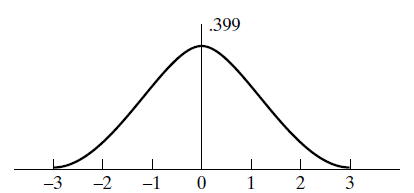
\includegraphics[scale=0.8]{figure4}
	\end{center}
	\label{reffig4}
	\caption{$\mu=0$, $\sigma=1$}
\end{figure}

$Z=\dfrac{X-\mu}{\sigma}$ is standard normally distributed with parameters $0$ and $1$.\\[0.5cm]
\indent{\itshape\bfseries Proof}\\[0.5cm]
Mean parameter
\begin{align*}
	E\left(\dfrac{X-\mu}{\sigma}\right) &=\dfrac{1}{\sigma}E(X-\mu)=\dfrac{1}{\sigma}[E(X)-E(\mu)]\\
	&=\dfrac{1}{\sigma}(\mu - \mu)=0.
\end{align*}
Volatility parameter
\begin{align*}
	Var\left(\dfrac{X-\mu}{\sigma}\right)
	&=\dfrac{1}{\sigma^2}Var(X-\mu)=\dfrac{1}{\sigma^2}[Var(X)-Var(\mu)]\\
	&=\dfrac{\sigma^2}{\sigma^2}=1.		
\end{align*}
The cumulative distribution function of standard normal random variable
\begin{align}
	\phi(x)&=\dfrac{1}{\sqrt{2\pi}} \displaystyle \int_{-\infty}^{x}e^\frac{-y^2}{2}dy \label{eq2.2.1} \\
	\phi(-x)&=1-\phi(x) \label{eq2.2.2}
\end{align}
\indent{\itshape\bfseries Proof}\\[0.5cm]
\indent Firstly, equation \eqref{eq2.2.1}\\
\indent Let $Y=\dfrac{X-\mu}{\sigma}$, then
\begin{align*}
	\phi(x)&=\displaystyle\int_{-\infty}^{x}\dfrac{1}{\sqrt{2\pi}\sigma}e^\frac{-(y-\mu)^2}{2\sigma^2}dy\\
	&=\displaystyle\int_{-\infty}^{x}\dfrac{1}{\sqrt{2\pi}\times1}e^\frac{-(y-0)^2}{2\times1^2}dy\\
	&=\dfrac{1}{\sqrt{2\pi}} \displaystyle \int_{-\infty}^{x}e^\frac{-y^2}{2}dy
\end{align*}
Secondly, equation \eqref{eq2.2.2} 
\begin{align*}
	\phi(-x)&=P\{X< -x\}\\
	&=P\{X> x\}\\
	&=P\{X\in (x,\infty)\}\\
	&=\dfrac{1}{\sqrt{2\pi}} \displaystyle \int_{x}^{\infty}e^\frac{-x^2}{2}dx\\
	&=\dfrac{1}{\sqrt{2\pi}} \displaystyle \int_{-\infty}^{\infty}e^\frac{-x^2}{2}dx - \dfrac{1}{\sqrt{2\pi}} \displaystyle \int_{-\infty}^{x}e^\frac{-x^2}{2}dx\\
	&=1 - \phi(x)
\end{align*}

\subsection{Lognormal property of stock price}
We have a random variable Y
\begin{center}
	$Y=e^X\sim$ $\log-N(\mu, \sigma^2)$ is distributed log-normally,\\ [0.3cm]
	then $\ln Y=X\sim N(\mu, \sigma^2)$ is normally distributed
\end{center}
The lognormal distribution is bounded below by $0$ and skewed to the right. It is extremely useful when analyzing stock prices which cannot fall below zero.
\begin{figure}[htp]
	\begin{center}
		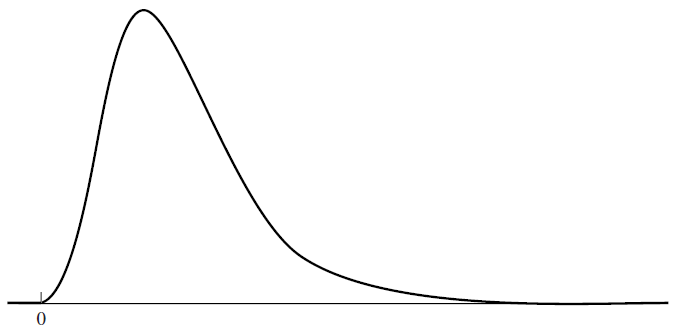
\includegraphics[scale=0.5]{figure7}
	\end{center}
	\label{reffig7}
	\caption{Lognormal distribution}
\end{figure}\\

\newpage
The mean value and variance of the log-normal distribution is given by
\begin{align}
	E(Y)&=e^{\mu+\frac{1}{2}\sigma^2} \label{eq2.3.1}\\
	Var(Y)&=e^{2\mu+\sigma^2}(e^{\sigma^2} - 1) \label{eq2.3.2}
\end{align}
%\indent{\itshape\bfseries Proof}\\[0.5cm]
%\indent Firstly, equation \eqref{eq2.3.1}\\ [0.5cm]
%$Y=e^X$ where $X$ is $N[\mu, \sigma^2]$. First, assuming that $\mu=0$
%\begin{align*}
%	E(Y)&=E(e^X)\\
%	&=\displaystyle \int_{-\infty}^{\infty}e^x \dfrac{1}{\sqrt{2\pi}\sigma}e^\frac{-x^2}{2\sigma^2}dx\\
%	&=\displaystyle \int_{-\infty}^{\infty}\dfrac{1}{\sqrt{2\pi}\sigma}e^\frac{2x\sigma^2 - x^2}{2\sigma^2}dx\\
%	&=\displaystyle \int_{-\infty}^{\infty}\dfrac{1}{\sqrt{2\pi}\sigma}e^\frac{-(x-\sigma^2)^2 + \sigma^4}{2\sigma^2}dx\\
%	&=e^\frac{\sigma^2}{2} \dfrac{1}{\sqrt{2\pi}\sigma}e^\frac{-(x-\sigma^2)^2}{2\sigma^2}dx\\
%	&=e^\frac{\sigma^2}{2}\times1 \\
%	&=e^\frac{\sigma^2}{2}
%\end{align*}
\begin{itemize}
	\item The probability density function of $LN(\mu, \sigma^2)$ is 
	\begin{center}
		$f(x)=\dfrac{1}{x\sqrt{2\pi}\sigma}e^\frac{-(lnx-\mu)^2}{2\sigma^2}$
	\end{center}
	\item The cumulative distribution function of $LN(\mu, \sigma^2)$ is
	\begin{align*}
		\displaystyle \int_{0}^{\infty}f(x)dx&=\dfrac{1}{x\sqrt{2\pi}\sigma} \displaystyle \int_{0}^{\infty}e^\frac{-(\ln x-\mu)^2}{2\sigma^2}dx\\
		&=\dfrac{1}{\sqrt{2\pi}\sigma} \displaystyle \int_{-\infty}^{\infty}e^\frac{-(y-\mu)^2}{2\sigma^2}dy\\
		&=1.
	\end{align*}
Where	$x=e^y$ or $lnx=y$, this leads to $\dfrac{dx}{x} = dy$	   
\end{itemize}
%Consider the continuously compounded rate of return between times 0 and T, $S_T$ is a lognormal distribution random variable. If the rate of return $r$ is continuously compounded then the future stock price can be expressed as 
%\begin{equation}
%	S_T = S_0 e^{rT} \label{2.3.3}
%\end{equation}
%Or
%\begin{align*}
%	\dfrac{S_T}{S_0} &= e^{rT}\\
%	ln\dfrac{S_T}{S_0} &= rT
%\end{align*}
%The continuously compounded rate of return between times 0 and T is normally distributed.\\
We consider the stock price $S_t$ as a random process which is only nonnegative. $S_T$ is the stock price at a future time $T$ and $S_0$ is the stock price at time $0$.  The variable $\ln S_T$ is normally distributed, so that $S_T$ has a
lognormal distribution. The mean of $\ln S_T$ is $\ln S_0+(\mu -\dfrac{\sigma^2}{2})T$ and the standard
deviation of $\ln S_T$ is $\sigma\sqrt{T}$. These are expressed by
\begin{align}
	\ln S_T \sim \phi[\ln S_0 + (\mu - \dfrac{\sigma^2}{2})T, \sigma^2T] \label{2.3.5}
\end{align}
Given an example for the expression \refeq{2.3.5}. Consider a stock with an initial price $S_0$ of $\$40$, an expected return $\mu$ of $16\%$ per
annum, and a volatility $\sigma$ of $20\%$ per annum. The probability
distribution of the stock price $S_T$ in $6$ months’ time is given by
\begin{align*}
	\ln S_T &\sim \phi[\ln 40 + (0.16 - 0.2^2/2)\times 0.5, 0.2^2\times 0.5]\\
	\ln S_T &\sim \phi(3.759, 0.02)
\end{align*}
There is a $95\%$ probability that a normally distributed variable has a value within
1.96 standard deviations of its mean. Therefore, the interval of stock price be able variation with $95\%$ confidence,
\begin{align*}
	3.759-1.96\times 0.141 \hspace{0.1cm}<\hspace{0.1cm} \ln S_T\hspace{0.1cm} <\hspace{0.1cm} 3.759+1.96\times 0.141
\end{align*}
This can be written
\begin{align*}
	e^{3.759-1.96\times 0.141}\hspace{0.1cm}<\hspace{0.1cm} S_T\hspace{0.1cm} <\hspace{0.1cm} e^{3.759+1.96\times 0.141}
\end{align*} 
Or
\begin{align*}
32.55\hspace{0.1cm}<\hspace{0.1cm} S_T \hspace{0.1cm}<\hspace{0.1cm} 56.56
\end{align*} 
Thus, there is a $95\%$ probability that the stock price in 6 months will lie between
$\$32.55$ and $\$56.56$.
%\indent{\itshape\bfseries %More explaination}
%\begin{align*}
%	X+a &\sim \phi(\mu + a, \sigma)\\
%	E(X+a) &= E[X]+E[a]\\
%	&=\mu + a\\
%	Var(X+a) &=Var(X)+ Var(a)\\
%	&=Var(X)
%\end{align*}
\section{Wiener Process}

In mathematics, a Wiener process is a stochastic process sharing the same behaviour as Brownian
motion, which is a physical phenomenon of random movement of particles suspended in a fluid. These financial models are
stochastic and continuous in nature, the Wiener process is usually employed to express the
random component of the model.

\subsection{Standard Wiener Process}
Let $(\Omega,\mathcal{F},\mathbb{P})$ be a probability space. A stochastic process $\{W_t ∶ t \geq 0\}$ is defined to be a standard Wiener process (or $\mathbb{P}$-standard Wiener process) if:
\begin{enumerate}
	\item $W_0 = 0$;
	\item With probability 1, the function $t \to W_t$ is continuous in t.
	\item The process $\{W_t\}_{t\geq 0}$ stationary, independent increments. 
	\item The increment $W_{t+s}-W_s$ has the normal distribution $\mathcal{N}(0,t)$.
\end{enumerate}
The term independent increments means that for every choice of nonnegative real numbers
\begin{align*}
0\leq s_1 < t_1 \leq s_2 < t_2 \leq \dots \leq s_n < t_n <\infty,
\end{align*}
the increment random variables
\begin{align*}
	W_{t_1}-W_{s_1}, W_{t_2}-W_{s_2},\dots, W_{t_n}-W_{s_n}
\end{align*}
are jointly independent; the term stationary increments means that for any $0 < s, t <\infty $ the distribution
of the increment $W_{t+s} −W_s$ has the same distribution as $W_t −W_0=W_t$.
\subsection{Martingale Pricing Theory}
Martingale pricing is a pricing approach based on the notions of equivalent martingale measure and risk-neutral valuation. The martingale pricing approach is a cornerstone of modern quantitative finance and can be applied to a form of derivatives contracts, e.g. options, future, etc. Without loss of generality, assume we are in the Black–Scholes world with an economy consisting of a risky asset or stock $S_t$ following a geometric Brownian
motion and a risk-free asset $B_t$ growing at a continuously compounded interest rate $r$ of the form\\
\begin{align*}
\dfrac{dS_t}{S_t}=\mu dt+\sigma dW_t, \hspace{0.3cm} \dfrac{dB_t}{B_t}=rdt
\end{align*}
where $\mu$ is the stock drift, $\sigma$ is the stock volatility and $W_t$ is a standard Wiener process on the
probability space $(\Omega, \mathcal{F}, \mathbb{P})$.

\subsubsection*{Radon–Nikody'm Theorem}
Let $(\Omega,\mathcal{F},\mathbb{P})$ be the probability space satisfying
the usual conditions. Let $\mathbb{Q}$ be another probability measure on $(\Omega,\mathcal{F},\mathbb{Q})$. Under the assumption
that $\mathbb{Q} << \mathbb{P}$, there exists a non-negative random variable $Z$ such that
\begin{align*}
	\dfrac{d\mathbb{Q}}{d\mathbb{P}}=Z
\end{align*}
and we call $Z$ the Radon–Nikody'm derivative of $\mathbb{Q}$ with respect to $\mathbb{P}$.\\[0.5cm]
Let's consider the standard Brownian process $Z_\mathbb{P}(t)$ under the measure $\mathbb{P}$.
Adding the drift $\mu t$ to $Z_\mathbb{P}(t)$, $\mu$ is a constant, we write
\begin{align*}
	Z_\mathbb{Q}(t)=Z_\mathbb{P}(t)+\mu t
\end{align*}
Here, $Z_\mathbb{Q}(t)$ is a Brownian process with drift under $\mathbb{P}$. we can change from
measure $\mathbb{P}$ to another measure 
$\mathbb{Q}$ so that $Z_\mathbb{Q}(t)$ becomes a Brownian process with
zero drift under 
$\mathbb{Q}$. Formally, we multiply $d\mathbb{P}$ by a factor $\dfrac{d\mathbb{Q}}{d\mathbb{P}}$ to give $d\mathbb{Q}$. It is postulated that the corresponding
Radon–Nikodym derivative for this case is given by
\begin{align}
	\dfrac{d\mathbb{Q}}{d\mathbb{P}} = e^{-\mu Z_\mathbb{P}(t)-\frac{\mu^2}{2}t } \label{Radon}
\end{align} 
When the drift rate is not constant, then The Girsanov Theorem presented below provides the Radon–Nikodym derivative.

\subsubsection*{Girsanov's Theorem}

Let $\{W_t :0 \leq t \leq T \}$ be a $\mathbb{P}$-standard Wiener process on the probability space $(\Omega, \mathcal{F}, \mathbb{P})$ and let $\mathcal{F}$, $0 \leq t \leq T$ be the associated Wiener process filtration. Suppose $\theta_t$ is an adapted process, $0 \leq t \leq T$ and consider
\begin{align*}
Z_t=e^{-\int_{0}^{t}\theta_sdW_s-\frac{1}{2}\int_{0}^{t}\theta_s^2ds}.
\end{align*}
Where $\{Z_t\}_{t \in [0,\infty)}$ be the
corresponding density process and if
\begin{align*}
\mathbb{E}^\mathbb{P}\left(e^{\frac{1}{2}\int_{0}^{T}\theta_s^2ds}\right)< \infty
\end{align*}
then $Z_t$ is a positive $\mathbb{P}$-martingale for $0 \leq t \leq T$ . By changing the measure $\mathbb{P}$ to a measure $\mathbb{Q}$
such that
\begin{align*}
\mathbb{E}^\mathbb{P}\left(\dfrac{d\mathbb{Q}}{d\mathbb{P}}\bigg| \mathcal{F}_t\right)=\dfrac{d\mathbb{Q}}{d\mathbb{P}}\bigg|_{\mathcal{F}_t}=Z_t
\end{align*}

then $W_t^\mathbb{Q} = W_t+\int_{0}^{t}\theta_udu$ is a $\mathbb{Q}$-standard Wiener process.\\ \vspace{0.4cm}

\textbf{Remark} Consider the stochastic differential equation (SDE)
\begin{align*}
dX_t=\mu(X_t,t)dt+\sigma(X_t,t)dW_t
\end{align*}
with $\mathbb{E}[(\displaystyle \int_{0}^{t}\sigma(X_s,s)^2ds)^2]\hspace{0.1cm}< \hspace{0.1cm}\infty$,then $X_t$ is a martingale if and only if $X_t$ is driftless (i.e., $\mu(X_t,t)=0$). Applying It\=o's quotient rule, 
\begin{align*}
\dfrac{d\left(\dfrac{S_t}{B_t}\right)}{\left(\dfrac{S_t}{B_t}\right)}&=\dfrac{dS_t}{S_t}-\dfrac{dB_t}{B_t}-\dfrac{dS_t}{S_t}\dfrac{dB_t}{B_t}+\left(\dfrac{dB_t}{B_t}\right)^2\\
&=(\mu-r)dt+\sigma dW_t
\end{align*}
and by writing $d W_t^\mathbb{Q}=dW_t+\theta dt$ where $\theta$ is a constant and $W_t^\mathbb{Q}$ a $\mathbb{Q}$-standard Wiener process, and applying Girsanov’s theorem to $d\left(\dfrac{S_t}{B_t}\right)/\left(\dfrac{S_t}{B_t}\right)$, we obtain
\begin{align*}
\dfrac{d\left(\dfrac{S_t}{B_t}\right)}{\left(\dfrac{S_t}{B_t}\right)}&=(\mu-r)dt+\sigma(dW_t^\mathbb{Q}-\theta dt)\\ 
&= (\mu-r-\theta\sigma)dt+\sigma d W_t^\mathbb{Q}
\end{align*}
To make $S_t/B_t$ a $\mathbb{Q}$-martingale, we set
\begin{align*}
\theta=\dfrac{\mu-r}{\sigma}.
\end{align*}
Thus, there is a unique $\theta$ which makes the discounted asset price process driftless, which is
equivalent to saying that there is a unique change of measure which makes the discounted asset
price a martingale under the risk-neutral measure.\\
\indent Hence, under the risk-neutral measure $\mathbb{Q}$, the asset price follows the diffusion process
\begin{align*}
\dfrac{dS_t}{S_t}&=\mu dt+\sigma dW_t\\
&=\mu dt +\sigma( dW_t^\mathbb{Q} - \theta dt)\\
&=\mu dt +\sigma( d W_t^\mathbb{Q}-\dfrac{\mu - r}{\sigma}dt)\\
&=rdt+\sigma d W_t^\mathbb{Q}
\end{align*}
%and solving the SDE for $T$ \textgreater \hspace{0.1cm}$t$ and under the filtration $\mathcal{F}_t$ we have
%\begin{align*}
%\textnormal{log}\left(\dfrac{S_T}{S_t}\right)\mid\mathcal{F}_t \sim \mathcal{N}((r-\frac{1}{2}\sigma^2)(T-t),\sigma^2(T-t)).
%\end{align*}
%Thus, the European call option at time $t$ with strike price K and expiry time $T$ \textgreater \hspace{0.1cm}$t$ is 
%\begin{align*}
%C(S_t, t; K, T) &= e^{-r(T-t)}\mathbb{E}^\mathbb{Q}\left[\textnormal{max}\{S_T-K,0\}\mid {\mathcal{F}_t}\right] \\
%&=e^{-r(T-t)}\mathbb{E}^\mathbb{Q}\left[(S_T-K,0)\mathcal{H}_{\{S_T \geq K\}} \mid {\mathcal{F}_t}\right] \\
%&=e^{-r(T-t)}\left\{\mathbb{E}^\mathbb{Q}\left[S_T\mathcal{H}_{\{S_T \geq K\}} \mid {\mathcal{F}_t}\right] -K\mathbb{E}^\mathbb{Q}\left[\mathcal{H}_{\{S_T \geq K\}} \mid {\mathcal{F}_t}\right]\right\}\\
%&=e^{-r(T-t)}\left\{\mathbb{E}^\mathbb{Q}\left[S_T\mathcal{H}_{\{S_T \geq K\}} \mid {\mathcal{F}_t}\right] -K\mathbb{Q}(S_T \geq K \mid {\mathcal{F}_t})\right\}
%\end{align*}

\subsubsection*{Equivalent Martingale Measure}

Let $(\Omega, \mathcal{F}, \mathbb{P})$ be the probability space
satisfying the usual conditions and let $\mathbb{Q}$ be another probability measure on $(\Omega, \mathcal{F}, \mathbb{P})$. The
probability measure $\mathbb{Q}$ is said to be an equivalent measure or risk-neutral measure if it satisfies
\begin{itemize}
	\item $\mathbb{Q} \sim \mathbb{P}$. This means that $\mathbb{Q}$ is equivalent to $\mathbb{P}$, if an
	event cannot occur under the $\mathbb{P}$ measure then it also cannot occur under the $\mathbb{Q}$ measure and
	vice versa $(\mathbb{Q}(\beta)=0\leftrightarrow \mathbb{P}(\beta)=0)$. Where $\beta$ is a random variable.  
	\item The discounted  risky asset price process $\{B_t^{-1}S_t^{(i)}\}, i=1,2,\mathellipsis, m $ are martingales under $\mathbb{Q}$, that is
	\begin{align*}
	\mathbb{E}^{\mathbb{Q}}(B_u^{-1}S_u^{(i)}| \mathcal{F}_t)=B_t^{-1}S_t^{(i)}
	\end{align*}
	for all $0 \leq t \leq u \leq T$. The equivalent martingale measure is a probability mesure such that each asset price is exactly equal to the discounted expectation of the asset price under $\mathbb{P}$. Moreover, the next step for all further steps, the expectation is equal to the current value given the available information $\mathcal{F}_t$. 
\end{itemize}
Let's look at an example of martingale, a fair gambling game. Let $K_0$ be the starting capital of a player. $X_i$ is the random profit of round i (can be negative, positive and zero). This implies the capital of the player after round one is $K_1=K_0+X_1$. In general after round $n$ the capital is $K_n=K_0+\sum_{i=1}^{n}X_i$. In a fair gambling game the expected profit is zero $\Rightarrow \mathbb{E}[X_i]=0$ for all $i\in \mathbb{N}$.\\
After $n$ rounds the values $K_0, K_1, \dots ,$ are known. If the profit in round $n+1$ is independent of the observed game then the expected capital is $K_{n+1}=K_n+X_{n+1}$. This implies
\begin{align*}
	\mathbb{E}[K_{n+1}|K_0,\dots,K_n]&=\mathbb{E}[K_{n}|K_0,\dots,K_n]+\mathbb{E}[X_{n+1}|K_0,\dots,K_n]\\
	&=K_n+\mathbb{E}[X_{n+1}]=K_n
\end{align*}
$\Rightarrow := (K_i)_{i\in \mathbb{N}}$ is a martingale. 
 
From the definition of an equivalent martingale measure, we can now state Girsanov’s theorem
which tells us how to convert from the real world $\mathbb{P}$ to the risk-neutral world $\mathbb{Q}$. We can change from a Wiener process with one drift $(\mu)$ to a standard Wiener process with another $(r)$.


\subsubsection*{Reflection Principle}
\fontsize{11pt}{20pt} \selectfont Let $(\Omega,\mathcal{F},\mathbb{P})$ be a probability space and let $\{W_t ∶ t \geq 0\}$ be a standard
Wiener process. By setting $\xi$ as a stopping time and defining a random process
\begin{align*}
\widetilde{W}_t= \begin{cases}
W_t \hspace{2cm}\textnormal{if} \hspace{0.2cm} t \hspace{0.1cm}  \textless \hspace{0.1cm}  \xi\\
2m-W_t \hspace{0.9cm}\textnormal{if} \hspace{0.1cm} \xi \hspace{0.1cm}  \leq \hspace{0.1cm}  t \hspace{0.1cm}  \leq \hspace{0.1cm} T,
\end{cases}
\end{align*}
that is, $\widetilde{W}_t$ is the mirror reflection of $W_t$ at the level $m$ within the time interval
between $\xi$ and $T$. It is then obvious that $\{W_T\hspace{0.1cm}> \hspace{0.1cm} x\}$ is equivalent to
$\{\widetilde{W}_T\hspace{0.1cm}< \hspace{0.1cm} 2m − x\}$, where $x\hspace{0.1cm} \geq \hspace{0.1cm} m$ and $ m \hspace{0.1cm}\leq \hspace{0.1cm} 0$  (see Fig. 2.5). 
\begin{figure}[htp]
	\begin{center}
		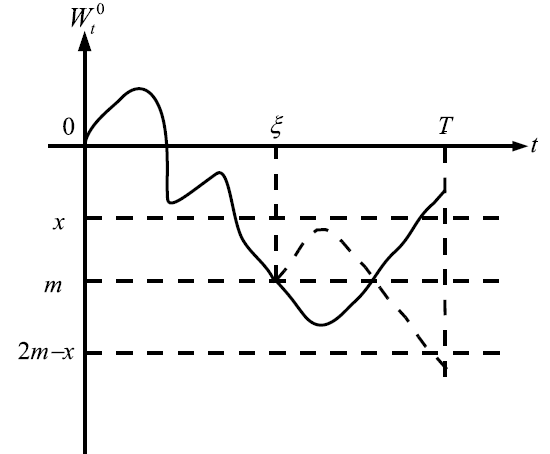
\includegraphics[scale=0.6]{figure5}
	\end{center}
	\label{reffig5}
	\caption{A graphical representation of the reflection principle of the Brownian motion $W_t$.}
\end{figure}

\newpage 
The dotted path after time $\xi$ is the mirror reflection of the Brownian path at the level m.
Suppose $W_T$ ends up at a value higher than x, then the reflected path at time $T$ has a value
lower than $2m − x$.

\subsubsection*{Quadratic Variation}

The quadratic varivation property of Bownian motion
\begin{itemize}
	\item $(dW_t)^2=dt$
	\item $dW_tdt=0$
	\item $(dt)^2=0$
	\item $(dW_t)^p=0, \hspace{0.3cm}p\geq3$
\end{itemize}\
Where ${W_t:t\geq 0}$ is a standard Brownian motion and $dW_t$ and $dt$ are the infinitesimal increment of $W_t$ and $t$, respectively. The significance of the above results constitutes the key ingredients in It\=o's formula to find the differential of a stochastic function and also in deriving the Black-Scholes equation to price option.
\subsubsection*{Geometric Brownian Motion}

The stock price cannot be negative (it is actually always positive, it just turns to zero when its company goes bankrupt). The stock price cannot be Browninan because the cycle of Brownian motion go to negative . But if we take logarithms of the stock price, it can be negative, and it can be imagined that the movement period  of the logarithms of the stock price  under the effect of random effects immediately on the market is similar to is the Browninan movement. Therefore, the following geometric Brownian motion concept is very important in describing the volatility of stock prices.\\[0.5cm]
GBM is the continuous time stochastic process $S_t$, which is defined by 
\begin{align*}
S_t=S_0e^{X_t} \label{x}
\end{align*}
where $X_t$ is Brownian motion with drift and $S(0)=S_0 \hspace{0.1cm} > \hspace{0.1cm} 0$ is the initial value. \\
The usual model for the time-evolution of an asset price $S_t$ is given by the GBM, represented by the following stochastic differential equation:
\begin{align*}
\dfrac{dS_t}{S_t}=\mu dt+\sigma dW_t
\end{align*}
The coefficients $\mu$ and $\sigma$, representing the drift and volatility of the asset, respectively, are both constant in this model.  \\[0.5cm]
Applying Taylor's theorem.\\[0.5cm]
Let $f(x)=\log S_t$
\begin{align*}
d(\log S_t)=df(x)=f^{\prime}(x)dx+\dfrac{1}{2}f^{\prime \prime}(x)dx^2=\dfrac{1}{x}dx+\dfrac{1}{2}(-\dfrac{1}{x^2})dx^2
\end{align*}
This leads to
\begin{align*}
d(logS_t)&=\dfrac{1}{S_t}dS_t+\dfrac{1}{2}\left(-\dfrac{1}{S_t^2}\right)dS_t^2\\
&=\dfrac{1}{S_t}(\mu S_tdt+\sigma S_tdW_t)-\dfrac{1}{2}\dfrac{(\mu S_tdt+\sigma S_tdW_t)^2}{S_t^2}\\
&=\mu dt+\sigma dW_t-\dfrac{1}{2}\dfrac{\sigma^2S_t^2dW_t^2}{S_t^2}\\
&=\mu dt+\sigma dW_t-\dfrac{\sigma^2dt}{2}\\
&=(\mu-\dfrac{\sigma^2}{2})dt+\sigma dW_t
\end{align*}
It is a standard Brownian motion with a drift term. Taking integral of  2 sides between the limits $0$ and $t$ we can write this as:
\begin{align*}
\int_{0}^{t}d(logS_u)&=\int_{0}^{t}\left(\mu -\dfrac{1}{2}\sigma^2 \right)u+\int_{0}^{t}\sigma W_u\\
logu|_0^t&=\left(\mu -\dfrac{1}{2}\sigma^2 \right)u\mid_0^t+\sigma W_u\mid_0^t\\
logS_t-logS_0&=\left(\mu -\dfrac{1}{2}\sigma^2 \right)(t-0)+\sigma(W_t-W_0)\\
logS_t-logS_0&=\left(\mu -\dfrac{1}{2}\sigma^2 \right)t+\sigma W_t\\
log\dfrac{S_t}{S_0}&=\left(\mu -\dfrac{1}{2}\sigma^2 \right)t+\sigma W_t
\end{align*}
Finally, taking the exponential of this equation gives:
\begin{align}
S_t=S_0e^{\left(\mu -\frac{1}{2}\sigma^2 \right)t+\sigma W_t}
\end{align} \label{eq2}

\section{Stochastic Differential Equations}

\textnormal A stochastic differential equation (SDE) is a differential equation in which one or more of
the terms has a random component. Within the context of mathematical finance, SDEs are
frequently used to model diverse phenomena such as stock prices, interest rates or volatilities
to name but a few. Typically, SDEs have continuous paths with both random and non-random
components and to drive the random component of the model they usually incorporate a Wiener
process.\\[0.5cm]
To begin with, a one-dimensional stochastic differential equation can be described as
\begin{align*}
dX_t=\mu(X_t,t)dt+\sigma(X_t,t)dW_t
\end{align*} 
where $W_t$ is a standard Wiener process, $\mu(X_t, t)$ is defined as the drift and $\sigma(X_t, t)$ the volatility.
Many financial models can be written in this form, such as the lognormal asset random walk,
common spot interest rate and stochastic volatility models.

\subsection{It\=o's lemma}
Ito's Lemma is a key component in the Ito Calculus, used to determine the derivative of a time-dependent function of a stochastic process.It can be heuristically derived by forming the Taylor series expansion of the function up to its second derivatives and retaining terms up to first order in the time increment and second order in the Wiener process increment. The lemma is widely employed in mathematical finance, and its best known application is in the derivation of the Black–Scholes equation for option values. Therefore, in order to derive It\=o's lemma we have to expand a Taylor series and applying the rules of stochastic calculus.

\subsubsection*{Taylor's Theorem}

Taylor's theorem in one real variable. \\
Let $k \geq 1$ be an integer and let the function $f : \mathbb{R} \to \mathbb{R}$ be $k$ times differentiable at the point $x_0 \in \mathbb{R}$ such that 
\begin{align*}
f(x)=f(x_0)+f^{\prime}(x_0)(x-x_0)+\dfrac{f^{\prime \prime}(x_0)}{2!}(x-x_0)^2+\dots+\dfrac{f^{(k)}(a)}{k!}(x-x_0)^k
\end{align*}
The partial derivatives through order 2 is given by
\begin{align*}
f(x)&=f(x_0)+f^{\prime}(x_0)(x-x_0)+\dfrac{f^{\prime \prime}(x_0)}{2!}(x-x_0)^2\\
f(x)-f(x_0)&=f^{\prime}(x_0)(x-x_0)+\dfrac{f^{\prime \prime}(x_0)}{2!}(x-x_0)^2\\
\Delta f(x)&=f^{\prime}(x_0)\Delta x+\dfrac{f^{\prime \prime}(x_0)}{2!}(\Delta x)^2
\end{align*}
When $\Delta x \rightarrow 0$ and $\Delta f(x) \rightarrow 0$.  This implies that
\begin{align*}
df(x)&=f^{\prime}(x)dx+\dfrac{1}{2}f^{\prime \prime}(x)dx^2
\end{align*}
Taylor's theorem in two real variable.  The partial derivatives of $f(x,t)$ through order 2 is 
\begin{align*}
df(x,t)=f^{\prime}_x(x,t)dx+f^{\prime}_t(x,t)dt+\dfrac{1}{2}f^{\prime \prime}_{x^2}(x,t)dx^2+\dfrac{1}{2}f^{\prime \prime}_{t^2}dt^2+f^{\prime \prime}_{xt}dxdt
\end{align*} 

\subsubsection*{Proof of It\=o's lemma}

Suppose that $f(X_t, t)$ is a continuous differential function of $t$ and $X_t$ follows 
\begin{align*}
dX_t=\mu_tdt+\sigma_tdW_t
\end{align*}
where $W_t$ is the Brownian motion. The variable $X_t$ has a drift rate of $\mu_t$ and has a variance rate of  $\sigma_t^2$. Applying Taylor's theorem in two variables $X_t$ and t we get
\begin{align*}
df(X_t,t)&=f^{\prime}_x(X_t,t)dX_t+f^{\prime}_t(X_t,t)dt+\dfrac{1}{2}f^{\prime \prime}_{x^2}(X_t,t)dX_t^2+\dfrac{1}{2}f^{\prime \prime}_{t^2}dt^2+f^{\prime \prime}_{xt}dX_tdt\\
\end{align*}
Based on the above quaratic variation property of Brownian motion we can obtain
\begin{align*}
df(X_t,t)&=f^{\prime}_x(X_t,t)dX_t+f^{\prime}_t(X_t,t)dt+\dfrac{1}{2}f^{\prime \prime}_{x^2}(X_t,t)dX_t^2+\dfrac{1}{2}f^{\prime \prime}_{t^2}0+f^{\prime \prime}_{xt}0\\
&=f^{\prime}_x(X_t,t)dX_t+f^{\prime}_t(X_t,t)dt+\dfrac{1}{2}f^{\prime \prime}_{x^2}(X_t,t)dX_t^2\\
&=f^\prime_x(X_t,t)(\mu_tdt+\sigma_tdW_t)+f^\prime_t(X_t,t)dt+\dfrac{1}{2}f^{\prime \prime}_{x^2}(X_t,t)(\mu_tdt+\sigma_tdW_t)^2\\
&=\left(f^\prime_t(X_t,t)+ \mu_tf^\prime_x(X_t,t)+\dfrac{\sigma_t^2}{2}f^{\prime \prime}_{x^2}(X_t,t)\right)dt+\sigma_t f^\prime_x(X_t,t)dW_t
\end{align*} 
Therefore, It\=o's lemma shows that a function $f$ of $X$ and $t$ follows the process 
\begin{align*}
df(X_t, t)=\left(\dfrac{\partial f}{\partial t}+\mu_t\dfrac{\partial f}{\partial x}+\dfrac{\sigma_t^2}{2}\dfrac{\partial^2 f}{\partial x^2}\right)dt+\sigma_t\dfrac{\partial f}{\partial x}dW_t
\end{align*}
\subsection{The Feynman-Kac formula}

Let $\{W_t: t \geq 0\}$ be a standard Wiener process on the probability space $(\Omega, \mathcal{F}, \mathbb{P})$ and let $\mathcal{F}_t$, $t \geq 0$ be the associated filtration. Let $X_t$ be the solution of the following SDE:
\begin{align*}
dX_t=\mu(X_t,t)dt+\sigma(X_t,t)dW_t
\end{align*} 
and define $r$ as a function of $t$. For $t\in [0,T]$ where $T \textgreater 0$ and if $V(X_t,t)$ satisfies the PDE
\begin{align}
\dfrac{\partial V}{\partial t}(X_t,t)+\dfrac{1}{2}\sigma(X_t,t)^2\dfrac{\partial^2V}{\partial X_t^2}(X_t,t)+\mu(X_t,t)\dfrac{\partial V}{\partial X_t}(X_t,t)-r(t)V(X_t,t)=0 \label{eq5.3.1}
\end{align} 
subject to the boundary condition $V(X_T,T)=\Psi (X_T)$, the under the filtration $\mathcal{F}_t$ the solution of the PDF is given by 
\begin{align*}
V(X_t,t)=\mathbb{E} \left[e^{-\int_{t}^{T}r(u)du}\Psi (X_T)\bigg|\mathcal{F}_t\right]
\end{align*}
By substituting $r(u)=r$, a constant. The time-t value $V(X_t; t)$ can be written as
\begin{align}
V(X_t; t)=e^{-r(T-t)}\mathbb{E}^\mathbb{Q}\left[\Psi (X_T)\bigg|\mathcal{F}_t\right]\label{eq5.3.2}
\end{align} 



	\chapter{The Black - Scholes - Merton model}


\section{European Call Option Valuation}
\fontsize{11pt}{20pt}\selectfont Let $\{W_t : t\geq 0\}$ be a $\mathbb{P}$-standard Wiener process on the probability space ($\Omega$, $\mathcal{F}$, $\mathbb{P}$) and let the asset price $S_t$ follow a GBM with the following SDE \\
\begin{align*}
\dfrac{dS_t}{S_t}=\mu dt+\sigma dW_t
\end{align*}
where $\mu$ is the drift parameter and $\sigma$ is the volatility parameter. \\ \vspace{0.01cm}

We expected to express the time-t value $C(S_t, t)$ of a European call option following to the the Feynman-Kac formula, then $C(S_t, t)$ must be satisfied the equation (\refeq{eq5.3.1}). A European call option $C(S_t, t)$ which is described by It\=o' lemma is given by
\begin{align*}
dC(S_t, t)=\left(\dfrac{\partial C}{\partial t}+\mu_tS_t\dfrac{\partial C}{\partial S_t}+\dfrac{1}{2}\sigma^2 S_t^2\dfrac{\partial^2 C}{\partial S_t^2}\right)dt+\sigma_tS_t\dfrac{\partial C}{\partial S_t}dW_t
\end{align*}
Now consider  portfolio consisting of the call option and $\alpha$ stocks. Then the
cost of the portfolio is $C+\alpha S_t$. We get
\begin{align*}
d(C+\alpha S_t)=\left(\dfrac{\partial C}{\partial t}+\mu_tS_t\dfrac{\partial C}{\partial S_t}+\dfrac{1}{2}\sigma^2 S_t^2\dfrac{\partial^2 C}{\partial S_t^2}+\alpha\mu S_t\right)dt+\sigma_tS_t\left(\dfrac{\partial C}{\partial S_t}+\alpha\right)dW_t
\end{align*}
Now we let $\alpha=-\dfrac{\partial C}{\partial S_t}(S_t,t)$ to hedge away all risk in our portfolio.
\begin{align*}
d(C+\alpha S_t)=\left(\dfrac{\partial C}{\partial t}+\dfrac{1}{2}\sigma^2 S_t^2\dfrac{\partial^2 C}{\partial S_t^2}+\alpha\mu S_t\right)dt
\end{align*}
As one can see, the random component $dW_t$, is now gone. The portfolio has no risk, it must grow
over time at the risk-free rate $r$. Thus,
\begin{align*}
	\dfrac{d}{dt}(C+\alpha S_t)=r(C+\alpha S_t)=r(C-S_t\dfrac{\partial C}{\partial S_t})
\end{align*}
and
\begin{align*}
	r(C-S_t\dfrac{\partial C}{\partial S_t})dt=\left(\dfrac{\partial C}{\partial t}+\dfrac{1}{2}\sigma^2 S_t^2\dfrac{\partial^2 C}{\partial S_t^2}+\alpha\mu S_t\right)dt
\end{align*}
Rearranging gives us the result that $C(S_t, t)$ follows the Keynman-Kac formula
\begin{align*}
	\dfrac{\partial C}{\partial t}(S_t, t)+rS_t\dfrac{\partial C}{\partial S_t}+\dfrac{1}{2}\sigma^2S_t^2\dfrac{\partial^2C}{\partial S^2}(S_t, t)-rC=0
\end{align*}
This means that the time-t value $C(S_t, t)$ can be written as
\begin{align}
		C(S_t, t)=e^{-r(T-t)}\mathbb{E}^\mathbb{Q}[C (S_T, T)|\mathcal{F}_t] \label{eq5.5.1}
\end{align}
\indent A European call option $C(S_t; t)$ written on $S_t$ with strike
price $K$ has the payoff $C(S_T ; T) = \textnormal {max}(S_T-K; 0)$. We substitute this payoff
in the Feynman-Kac formula in Equation \eqref{eq5.5.1}. Hence, the time-$t$ value of a
European call is
\begin{align*}
	C(S_t,t;K,T) = e^{-r(T-t)}\mathbb{E}^\mathbb{Q}[\textnormal{max}\{S_T-K,0\}\mid\mathcal{F}_t]
\end{align*}
%where $\mathbb{E}^\mathbb{Q}$(.) is the expectation under the risk-neutral measure $\mathbb{Q}$.
%Using the risk-neutral valuation approach show that the European call option price is
%\begin{align*}
%	C(S_t,t;K,T)=S_te^{-(T-t)}\Phi(d_+)-Ke^{-r(T-t)}\Phi(d_-) 
%\end{align*} 
%where
%\begin{align*}
%d_\pm=\dfrac{\textnormal{log}(S_t/K)+(r-\pm \frac{1}{2}\sigma^2)(T-t)}{\sigma \sqrt{T-t}}
%\end{align*}
%and $\Phi(x)$ is the standard normal cdf
%\begin{align*}
%\Phi(x)=\displaystyle \int_{-\infty}^{x}\dfrac{1}{2\pi} e^{-\frac{1}{2}u^2}du
%\end{align*}
%
%Expain
From Girsanov's theorem, under a $\mathbb{Q}$-standard Wiener process we have
\begin{align*}
W_t^\mathbb{Q}&=W_t+\left(\dfrac{\mu-r}{\sigma}\right)t \hspace{0.2cm} 
\end{align*}
%This leads to
%\begin{align*}
%dW_t^\mathbb{Q}&=dW_t+\left(\dfrac{\mu-r}{\sigma}\right)dt
%\end{align*} 
% Hence, under the risk-neutral measure $\mathbb{Q}$ the asset price follows the diffusion process
%\begin{align*}
%\dfrac{dS_t}{S_t}&=\mu dt+\sigma\left(W_t^\mathbb{Q}-\dfrac{\mu-r}{\sigma}t\right)\\
%&=\mu dt+\sigma dW_t^\mathbb{Q}-(\mu-r)dt\\
%&=rdt+\sigma dW_t^\mathbb{Q}
%\end{align*}
And consider equation \eqref{eq2} which has been appoved in property of GBM
\begin{align*}
S_t=S_0e^{\left(\mu -\frac{1}{2}\sigma^2 \right)t+\sigma W_t}
\end{align*}
Under the risk-neutral measure $\mathbb{Q}$, that equation is equivalent to
\begin{align}
S_t=S_0e^{\left(r -\frac{1}{2}\sigma^2 \right)t+\sigma W_t^{\mathbb{Q}}} \label{eq5.5.2}
\end{align} 
where $r$ is the risk-free interest rate. This implies that
\begin{align*}
S_t&=e^{logS_0}e^{\left(r -\frac{1}{2}\sigma^2 \right)t+\sigma W_t^{\mathbb{Q}}}\\
&=e^{logS_0+\left(r -\frac{1}{2}\sigma^2 \right)t+\sigma W_t^{\mathbb{Q}}}
\end{align*}

For $T\hspace{0.1cm}>t\hspace{0.1cm}$, $W_{T-t}^\mathbb{Q} \sim \mathcal{N}(0, T-t)$. Hence, conditional on $S_t$ we can write
\begin{align*}
	S_T \mid S_t\sim \textnormal{log}-\mathcal{N}[\textnormal{log}S_t+(r-\dfrac{1}{2}\sigma^2)(T-t),\sigma^2(T-t)]
\end{align*}
Under the risk-neutral measure $\mathbb{Q}$ we can write the European call option price as
\begin{align*}
C(S_t,t;K,T) &= e^{-r(T-t)}\mathbb{E}^\mathbb{Q}[\textnormal{max}\{S_T-K,0\}\mid\mathcal{F}_t]\\
			&=e^{-r(T-t)} \displaystyle \int_{0}^{\infty}\textnormal{max}\{S_T-K,0\}f(S_T\mid S_t)dS_t.
\end{align*}
Here, for a log normally distributed random variable log $X\sim \mathcal{N}(\mu, \sigma^2)$ the PDF is
\begin{align*}
f_X(x; \mu, \sigma)=\dfrac{1}{x\sigma\sqrt{2\pi}}e^{-\frac{1}{2}\left(\frac{\log x-\mu}{\sigma}\right)^2} \hspace{0.2cm},\hspace{0.2cm} x\hspace{0.1cm} > \hspace{0.1cm}0
\end{align*}
Since $S_T$ conditional on $S_t$ have drift is equal to $\log S_t+(r-\dfrac{1}{2}\sigma^2)(T-t)$  
and we can thus write
\begin{align*}
f(S_T | S_t)=\dfrac{1}{S_T\sigma\sqrt{2\pi(T-t)}}e^{-\frac{1}{2}\left(\frac{\log S_T-\log S_t-(r-\frac{1}{2}\sigma^2)(T-t)}{\sigma\sqrt{T-t}}\right)^2} \hspace{0.2cm},\hspace{0.2cm} S_T\hspace{0.1cm} > \hspace{0.1cm}0
\end{align*}
or
\begin{align*}
f(S_T| S_t)=\dfrac{1}{S_T\sigma\sqrt{2\pi(T-t)}}e^{-\frac{1}{2}\left(\frac{\log S_T-m}{\sigma\sqrt{T-t}}\right)^2} \hspace{0.2cm},\hspace{0.2cm} S_T\hspace{0.1cm} > \hspace{0.1cm}0
\end{align*}
where $m=\log S_t+(r-\frac{1}{2}\sigma^2)(T-t)$. Therefore,
\begin{align*}
C(S_t,t;K,T) =\hspace{0.1cm} &e^{-r(T-t)} \displaystyle \int_{0}^{K}\max\{S_T-K,0\}f(S_T| S_t)dS_t \\ 		       &+e^{-r(T-t)} \displaystyle \int_{K}^{\infty}\max\{S_T-K,0\}f(S_T| S_t)dS_t\\
			  =\hspace{0.1cm} &e^{-r(T-t)} \displaystyle \int_{K}^{\infty}(S_T-K)f(S_T| S_t)dS_t\\
			  =\hspace{0.1cm} &I_1-I_2
\end{align*}
where
\begin{align*}
I_1=e^{-r(T-t)} \displaystyle \int_{K}^{\infty}S_Tf(S_T| S_t)dS_t \hspace{0.3cm} \textnormal{and} \hspace{0.3cm} I_2=e^{-r(T-t)} \displaystyle \int_{K}^{\infty}Kf(S_T| S_t)dS_t
\end{align*}
Solving $I_1$ we have 
\begin{align*}
I_1 &=e^{-r(T-t)} \displaystyle \int_{K}^{\infty}S_Tf(S_T\mid S_t)dS_t\\
	&=e^{-r(T-t)} \displaystyle \int_{K}^{\infty}\dfrac{1}{\sigma\sqrt{2\pi(T-t)}}e^{-\frac{1}{2}\left(\frac{\textnormal{log}S_T-m}{\sigma\sqrt{T-t}}\right)^2}dS_t
\end{align*}
and by letting $u=\frac{\log S_T-m}{\sigma\sqrt{T-t}}$ we then have
\begin{align*}
	I_1=\dfrac{e^{m-r(T-t)}}{\sqrt{2\pi}}\displaystyle \int_{\frac{\log K-m}{\sigma\sqrt{T-t}}}^{\infty}e^{-\frac{1}{2}u^2+\sigma u\sqrt{T-t}}du.
\end{align*}
Using the sum of squares
\begin{align*}
	-\dfrac{1}{2}u^2+\sigma u\sqrt{T-t}=\dfrac{1}{2}\left[(u-\sigma\sqrt{T-t})^2-\sigma^2(T-t)\right]
\end{align*}
we can simplify $I_1$ to become
\begin{align*}
I_1&=\dfrac{e^{m-r(T-t)}}{\sqrt{2\pi}}\displaystyle \int_{\frac{\log K-m}{\sigma\sqrt{T-t}}}^{\infty}e^{-\frac{1}{2}\left[(u-\sigma\sqrt{T-t})^2-\sigma^2(T-t)\right]}du\\
&=\dfrac{e^{m-r(T-t)+\frac{1}{2}\sigma^2(T-t)}}{\sqrt{2\pi}}\displaystyle\int_{\frac{\log K-m}{\sigma\sqrt{T-t}}}^{\infty}e^{-\frac{1}{2}\left(u-\sigma\sqrt{T-t}\right)^2}du\\
&=e^A\left[\displaystyle\int_{-\infty}^{\infty}\dfrac{1}{\sqrt{2\pi}}e^{-\frac{1}{2}\left(u-\sigma\sqrt{T-t}\right)^2}du-\displaystyle\int_{-\infty}^{\frac{\log K-m}{\sigma\sqrt{T-t}}}e^{-\frac{1}{2}\left(u-\sigma\sqrt{T-t}\right)^2}du\right]
\end{align*}
Where 
\begin{align*}
	A&=m-r(T-t)+\frac{1}{2}\sigma^2(T-t)\\
	&=\log S_t+(r-\frac{1}{2}\sigma^2)(T-t) -r(T-t)+\frac{1}{2}\sigma^2(T-t)=\log S_t
\end{align*}
By setting $v=u-\sigma\sqrt{T-t}=\dfrac{\log(K/S_t)-(r-\frac{1}{2}\sigma^2)(T-t)}{\sigma\sqrt{T-t}}$ and substituting\\ $m=\log S_t+(r+\frac{1}{2}\sigma^2)(T-t)$ we have
\begin{align*}
	\displaystyle\int_{-\infty}^{\frac{\log K-m}{\sigma\sqrt{T-t}}}e^{-\frac{1}{2}\left(u-\sigma\sqrt{T-t}\right)^2}du = \displaystyle\int_{-\infty}^{\frac{\log(K/S_t)-(r+\frac{1}{2}\sigma^2)(T-t)}{\sigma\sqrt{T-t}}}e^{-\frac{1}{2}\nu^2}d\nu
\end{align*}
Therefore, 
\begin{align*}
	I_1&=e^{\log S_t}\left[1-\displaystyle\int_{-\infty}^{\frac{\log(K/S_t)-(r+\frac{1}{2}\sigma^2)(T-t)}{\sigma\sqrt{T-t}}}e^{-\frac{1}{2}\nu^2}d\nu\right]\\
	&=S_t\left[1-\Phi\left(\dfrac{\log(K/S_t)-(r+\frac{1}{2}\sigma^2)(T-t)}{\sigma\sqrt{T-t}}\right)\right]\\
	&=S_t\Phi\left(\dfrac{\log(S_t/K)+(r+\frac{1}{2}\sigma^2)(T-t)}{\sigma\sqrt{T-t}}\right).
\end{align*}
Similarly for $I_2$ we have
\begin{align*}
 I_2&=e^{-r(T-t)} \displaystyle \int_{K}^{\infty}Kf(S_T)dS_T\\
 	&=Ke^{-r(T-t)} \displaystyle \int_{K}^{\infty}\dfrac{1}{S_T\sigma\sqrt{2\pi(T-t)}}e^{-\frac{1}{2}\left(\frac{\log S_T-m}{\sigma\sqrt{T-t}}\right)^2}dS_T
\end{align*}
and by letting  $u=\frac{\log S_T-m}{\sigma\sqrt{T-t}}$ and substituting $m=\log S_t+(r-\frac{1}{2}\sigma^2)(T-t)$ \\
\begin{align*}
I_2&=e^{-r(T-t)}K \displaystyle \int_{\frac{\log K-m}{\sigma\sqrt{T-t}}}^{\infty}\dfrac{1}{\sqrt{2\pi}}e^{-\frac{1}{2}u^2}du\\
	&=Ke^{-r(T-t)}\left[1-\Phi\left(\frac{\log K-m}{\sigma\sqrt{T-t}}\right)\right]\\
	&=Ke^{-r(T-t)}\left[1-\Phi\left(\dfrac{\log(K/S_t)-(r-\frac{1}{2}\sigma^2)(T-t)}{\sigma\sqrt{T-t}}\right)\right]\\
	&=Ke^{-r(T-t)}\Phi\left(\dfrac{\log(S_t/K)+(r-\frac{1}{2}\sigma^2)(T-t)}{\sigma\sqrt{T-t}}\right)
\end{align*}
Therefore, 
\begin{align}
	C(S_t,t;K,T)=S_te^{-(T-t)}\Phi(d_1)-Ke^{-r(T-t)}\Phi(d_2) \label{eqBS}
\end{align}
where 
\begin{align*}
d_1&=\dfrac{\log(S_t/K)+(r+ \frac{1}{2}\sigma^2)(T-t)}{\sigma \sqrt{T-t}}\\
d_2&=\dfrac{\log(S_t/K)+(r- \frac{1}{2}\sigma^2)(T-t)}{\sigma \sqrt{T-t}}
\end{align*}

\section{Application}

\subsection{Condition of the Black-Sholes-Merton moldel}
Six assumptions of the Black-Sholes-Merton model is given by
\begin{enumerate}
	\item The option is European 
	\item No dividends are paid out during the option's life
	\item Efficient markets
	\item There are no transaction costs in buying the option
	\item The risk-free rate and volatility of the underlying are known and constant
	\item The returns on the underlying are normally distributed
\end{enumerate}
\subsubsection*{Problem}
Consider a European call option on FPT stock without dividends. Market movements cannot be predicted. These information is given $5$ first assumptions. We need to check the last one which is the rate of returns are normally distributed. We can get the historical data from source: \url{http://www.cophieu68.vn/historyprice.php?id=fpt}, the stock price is just calculated in 1  year, 2017. Firstly, we will compute daily return $(u_i) $ of FPT stock. 
\begin{align*}
	u_i=\ln\dfrac{S_i}{S_{i-1}} \hspace{0.4cm} \text{for}\hspace{0.2cm}i=0, 1, \dots, n
\end{align*}
where \\
$n+1$: Number of observations\\
$S_i$: Stock price at end of $i$th interval, with $i=0, 1, \dots, n$
\subsubsection*{Testing for normal distribution}
The software is using for testing data is R – Studio. The code is shown at the end of report. We will use graphical methods which is normal probability plot (Q-Q plot or quantile quantile plots).
Q-Q plot is a graphical technique to help us assess whether or not a data set is approximately normally distributed. %The question is how to make a Q-Q plot. The method is following  
%\begin{itemize}
%	\item Sort the numbers from smallest to largest
%	\item Draw a normal distribution curve
%	\item Find the Z-value for each segment
%	\item Plot data set value against the Z-value 
%\end{itemize}
If the most part the data points follow along the straight line, this will be normally distributed. We will describe the previous daily return.  Here is our result
\begin{figure}[htp]
	\begin{center}
		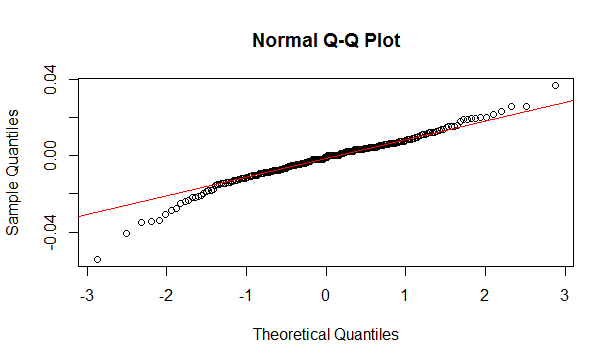
\includegraphics[scale=.8]{Rplot03}
	\end{center}
	\label{refRplot03}
	\caption{The distribution of FPT stock}
\end{figure}

\newpage
This graph satisfies conditions of normal distribution. Here the x-axis is the probability and the y-axis is the values of returns.
Therefore, the returns is most likely normally distribution.
\subsection{Apply to the Black-Scholes-Merton model}

Let's asumme that FPT stock satisfies conditions of the Black-Scholes-Merton model. We first estimate the volatility of a stock price empirically. The usual estimate, $s$, of the standard deviation of the $u_i$ is given by
\begin{align*}
	s&=\sqrt{\dfrac{1}{n-1}\sum_{i=1}^{n}(u_i-\bar{u})^2}
\end{align*}
or
\begin{align*}
 s=\sqrt{\dfrac{1}{n-1}\sum_{i=1}^{n}u_i^2-\dfrac{1}{n(n-1)}\left(\sum_{i=1}^{n}u_i\right)^2}
\end{align*}
where $\bar{u}$ is the mean of the $u_i$. An estimate for the volatility per annum as 
\begin{align*}
	\text{Volatility
	per annum} = \text{Volatility
	per trading day} \times \sqrt{\text{Number of trading days
		per annum}}
\end{align*}

\newpage
Using R-studio, we get 
\begin{itemize}
	\item Volatility
	per trading day $s = 0.015$
	\item There are 250 trading days of year 2017. Therefore,\\ Volatility
	per annum = $s\times \sqrt{250}$ = 24\%
\end{itemize}
This company currently sells for $59.8$ VND per share. The annual stock price volatility is $24\%$. Assume that the annual continuously compounded risk-free interest rate is $3\%$. Using the Black-Scholes model for the price of a call option on a company's stock with strike price $62$ VND and time for expiration of half a year. Let's cover it.
\begin{table}[!htp]
	\centering
	\begin{tabular}{|l|c|r|}
	\hline
	$S_0$ & Stock price at time zero   & $59.8$ VND\\
	\hline
	$K$ & Strike price  & $62$ VND\\
	\hline
	$\sigma$ &  Annual volitility & $24\%$\\
	\hline
	$r$ & Annual riskless rate  & $3\%$ \\
	\hline
	$T$ & Option expiration (in years)  & $0.5$\\
	\hline	
	\end{tabular}
	\caption{FPT stock}
	\label{B3.1}
\end{table}

We first calculate each components of equation \refeq{eqBS}. 
\begin{align*}
	d_1&=\dfrac{\log(S_0/K)+(r+ \frac{1}{2}\sigma^2)T}{\sigma \sqrt{T}}= -0.04\\
	d_2&=\dfrac{\log(S_0/K)+(r- \frac{1}{2}\sigma^2)T}{\sigma \sqrt{T}}=-0.21
\end{align*}
Substituting the above variables into equation \refeq{eqBS}, we get
\begin{align*}
	C(S_0,0;K,T)=S_0e^{-T}\Phi(d_1)-Ke^{-rT}\Phi(d_2)=3.48 
\end{align*}
This means that the option price or a premium is $3.48$ VND for each stock.
	
\chapter{European Barrier Options with Rebates}

\section{European Down and Out Call Option}

\fontsize{11pt}{20pt}\selectfont We require $S_t\hspace{0.1cm} > \hspace{0.1cm} B$ for all $t$ so as to ensure the option would not knock out at the starting
time $t$. Consider a case for the down-and-out call option price when $B \leq K$. In this case, the holder will get more payoff than $B \geq K$. the payoff of a down-and-out call option is
\begin{align*}
C_{d/o}(S_T)=\max\{S_T-K, 0\}\mathcal{H}_{\{min_{t\leq u\leq T}S_u > B\}}
\end{align*}
Under the risk-neutral measure $\mathbb{Q}$, $S_t$ follows
\begin{align*}
\dfrac{dS_t}{S_t}=rdt+\sigma dW_t^\mathbb{Q}
\end{align*}
such that $W_t^\mathbb{Q}=W_t+\left(\dfrac{\mu-r}{\sigma}\right)t$ \hspace{0.1cm}is a $\mathbb{Q}$-standard Wiener process. Following equation \eqref{eq5.5.2} with times from $t$ to $T$ for $T\hspace{0.1cm}>\hspace{0.1cm}t$, we obtain
\begin{align}
\begin{split}
S_T&=S_te^{\left(r -\frac{1}{2}\sigma^2 \right)(T-t)+\sigma W_{T-t}^\mathbb{Q}}\\
&=S_te^{\sigma \widehat{W}_{T-t}}
\end{split} \label{eq4.1.1}
\end{align} 
where $\widehat{W}_{T-t}=\nu (T-t)+W_{T-t}^\mathbb{Q}$ and $\nu=\dfrac{1}{\sigma}(r-\dfrac{1}{2}\sigma^2)$. By writing
\begin{align*}
	m_{T-t}=min_{t\leq u \leq T}\widehat{W}_{u-t}
\end{align*}
Therefore, 
\begin{align*}
\displaystyle \min_{t\leq u \leq T}S_u&=\displaystyle \min_{t\leq u \leq T}S_te^{\sigma \widehat{W}_{u-t}} \\
&=S_te^{\sigma \min_{t\leq u \leq T}\widehat{W}_{u-t}}\\
&=S_te^{\sigma 	m_{T-t}}
\end{align*} 
and we can rewrite the payoff as  \cite{Eric}
\begin{align*}
C_{d/o}(S_T)&=\max\{S_T-K, 0\}\mathcal{H}_{\{min_{t\leq u\leq T}S_u > B\}}\\
&=\max\{S_te^{\sigma \widehat{W}_{T-t}}-K, 0\}\mathcal{H}_{\{S_te^{\sigma 	m_{T-t}} > B, \}}\\
&=(S_te^{\sigma \widehat{W}_{T-t}}-K)\mathcal{H}_{\{S_te^{\sigma m_{T-t}} > B, S_te^{\sigma \widehat{W}_{T-t}}> K\}}\\
&=(S_te^{\sigma \widehat{W}_{T-t}}-K)\mathcal{H}_{\{m_{T-t}>\frac{1}{\sigma}\log\left(\frac{B}{S_t}\right), \widehat{W}_{T-t}>\frac{1}{\sigma}log\left(\frac{K}{S_t}\right) \}}
\end{align*}
The down-and-out call option price at time $t$ is
\begin{align*}
	C_{d/o}(S_t,t;K,B,T) &= e^{-r(T-t)}\mathbb{E}^\mathbb{Q}[C_{d/o}(S_T)|\mathcal{F}_t]\\
	&=e^{-r(T-t)}\mathbb{E}^\mathbb{Q}[(S_te^{\sigma \widehat{W}_{T-t}}-K)\mathcal{H}_{\{m_{T-t}>\frac{1}{\sigma}\log\left(\frac{B}{S_t}\right), \widehat{W}_{T-t}>\frac{1}{\sigma}\log\left(\frac{K}{S_t}\right) \}}\bigg|\mathcal{F}_t]\\
	&=e^{-r(T-t)}\displaystyle \int_{\omega =\frac{1}{\sigma}log\left(\frac{K}{S_t}\right) }^{\infty}\displaystyle \int_{m =\frac{1}{\sigma}log\left(\frac{B}{S_t}\right) }^{m=\omega}(S_te^{\sigma \omega}-K)f^\mathbb{Q}_{m,\widehat{W}}(m, \omega)dmd\omega
\end{align*}
where $f^\mathbb{Q}_{m,\widehat{W}}(m, \omega)$ is the joint probability density function of $(m, \widehat{W})$. We need to find out this function which is necessary for deriving the European barrier call option. \\ [0.5cm]
Given $m_t=\displaystyle \min_{0\leq t\leq T} W_t =-\displaystyle \max_{0\leq t\leq T}\{-W_t\}$ we have for $m\leq 0$ and $m\leq \omega$,
\begin{align*}
	\mathbb{P}(m_t\geq m, W_t \geq \omega)&=\mathbb{P}\left(-\displaystyle \max_{0\leq t\leq T}\{-W_t\}\geq m, W_t\geq \omega\right)\\
	&=\mathbb{P}\left(-\displaystyle \max_{0\leq t\leq T}\{-W_t\}\geq m, -W_t\leq -\omega\right)\\
	&= \mathbb{P}\left(\displaystyle \max_{0\leq t\leq T}{\widetilde{W}_t}\leq -m, \widetilde{W}_t\leq -\omega\right)
\end{align*}
where the last equality comes from the symmetric property of the standard Wiener process such that $\widetilde{W}_t=-W_t \sim \mathcal{N}(0, t)$ is also a standard Wiener process.\\
Since
\begin{align*}
	\mathbb{P}(\widetilde{W}_t\leq -\omega)=\mathbb{P}\left(\displaystyle \max_{0\leq t\leq T}{\widetilde{W}_t}\leq -m, \widetilde{W}_t\leq -\omega\right)+\mathbb{P}\left(\displaystyle \max_{0\leq t\leq T}{\widetilde{W}_t}\geq -m, \widetilde{W}_t\leq -\omega\right)
\end{align*}
We have
\begin{align}
\begin{split}
	\mathbb{P}\left(\displaystyle \max_{0\leq t\leq T}{\widetilde{W}_t}\geq -m, \widetilde{W}_t\leq -\omega\right)&=	\mathbb{P}\left(\displaystyle \min_{0\leq t\leq T}W_t \leq m, W_t\geq \omega\right)\\
	&=\mathbb{P}(\tilde{W}_t\hspace{0.1cm} >\hspace{0.1cm} 2m-\omega)\\
	&=\Phi\left(\dfrac{2m-\omega}{\sqrt{t}}\right)
	\end{split} \label{negative}
\end{align} 
Since T is finite, from Reflection Princciple and the strong Markov property both $W_t$ and $\tilde{W}_t$ are standard Wiener processes and independent which means that they have the same distribution.\\
We tend to the Brownian motion $W_t$ which has a downstream barrier $m$ over the period
$[0, T]$ so that $m_t \geq m$, we would like to derive the joint distribution
\begin{align}
		\mathbb{P}(m_t\geq m, W_t \geq \omega)&=\mathbb{P}\left(\displaystyle \max_{0\leq t\leq T}{\widetilde{W}_t}\leq -m, \widetilde{W}_t\leq -\omega\right) \nonumber\\
		&=\mathbb{P}(\widetilde{W}_t\leq -\omega)-\mathbb{P}\left(\displaystyle \max_{0\leq t\leq T}{\widetilde{W}_t}\geq -m, \widetilde{W}_t\leq -\omega\right) \nonumber \label{eq601}\\
		&=\Phi \left(-\dfrac{\omega}{\sqrt{t}}\right)-\Phi\left(\dfrac{2m-\omega}{\sqrt{t}}\right)
\end{align}
To obtain the joint probability density function by definition,
\begin{align*}
	f_{m_t,W_t}(m, \omega)&=\dfrac{\partial^2}{\partial m \partial \omega}\mathbb{P}(m_t\geq m, W_t \geq \omega)\\
	&=\dfrac{\partial^2}{\partial m \partial \omega}\left[\Phi\left(-\dfrac{\omega}{\sqrt{t}}\right)-\Phi\left(\dfrac{2m-\omega}{\sqrt{t}}\right)\right]\\
	&=\dfrac{\partial}{\partial m}\left[\dfrac{\partial}{\partial\left(-\frac{\omega}{\sqrt{t}}\right)}\Phi\left(-\dfrac{\omega}{\sqrt{t}}\right)\dfrac{\partial}{\partial \omega}\Phi\left(-\dfrac{\omega}{\sqrt{t}}\right)-\dfrac{\partial}{\partial\left(\frac{2m-\omega}{\sqrt{t}}\right)}\Phi\left(\dfrac{2m-\omega}{\sqrt{t}}\right)\dfrac{\partial}{\partial \omega}\Phi\left(\dfrac{2m-\omega}{\sqrt{t}}\right)\right]\\
	&=\dfrac{\partial}{\partial m}\left[-\dfrac{1}{\sqrt{2\pi t}}e^{-\frac{1}{2}\left(\frac{\omega}{\sqrt{t}}\right)^2}+\dfrac{1}{\sqrt{2\pi t}}e^{-\frac{1}{2}\left(\frac{2m-\omega}{\sqrt{t}}\right)^2}\right]\\
	&=\dfrac{-2(2m-\omega)}{t\sqrt{2\pi t}}e^{-\frac{1}{2}\left(\frac{2m-\omega}{\sqrt{t}}\right)^2}
\end{align*}
Moreover, for $m\geq 0$, since $m_t\leq W_0=0$ so $\mathbb{P}(m_t\geq m, W_t\geq \omega)=0$.\\
We obtain the joint probability distribution of $(m_t, W_t)$ under $\mathbb{Q}$ is
\begin{align*}
f^\mathbb{Q}_{m,W}(m, \omega)= \begin{cases}
\dfrac{-2(2m-\omega)}{t\sqrt{2\pi t}}e^{-\frac{1}{2t}(2m-\omega)^2} \hspace{0.2cm} &m\leq 0,m\leq \omega   \nonumber \\
	0 &\text{otherwise.}  \nonumber
\end{cases}
\end{align*}
In order to find the joint cumulative distribution function of $(m_t, W_t)$, we consider Girsanov’s theorem there exists an equivalent probability
measure $\mathbb{Q}$ on the filtration $\mathcal{F}_t$, $0 \leq s \leq t$ defined by the Radon–Nikody$^\prime$m derivative
\begin{align*}
	Z_s&=e^{-\int_{0}^{s}\alpha dW_u-\frac{1}{2}\int_{0}^{s}\alpha^2du}\\
	&=e^{-\alpha W_s-\frac{1}{2}\alpha^2s}\\
	&=e^{-\alpha(W_t^\mathbb{Q}-\alpha s)-\frac{1}{2}\alpha^2 s }\\
	&=e^{-\alpha W_t^\mathbb{Q}+\frac{1}{2}\alpha^2s}
\end{align*}
Let's  consider the joint CDF of $(m_t, W_t)$
\begin{align*}
		\mathbb{P}(m_t\leq m, W_t \leq \omega)&=\mathbb{E}^\mathbb{P}(\mathcal{H}_{\{m_t\leq m, W_t \leq \omega\}})\\
		&=\mathbb{E}^\mathbb{Q}(Z_t^{-1}\mathcal{H}_{\{m_t\leq m, W_t \leq \omega\}})\\
		&=\mathbb{E}^\mathbb{Q}(e^{\nu W_t^\mathbb{Q}-\frac{1}{2}\nu^2t}\mathcal{H}_{\{m_t\leq m, W_t \leq \omega\}})\\
		&=\displaystyle \int_{-\infty}^{\omega} \displaystyle \int_{-\infty}^{m}e^{\nu \omega-\frac{1}{2}\nu^2 t}f_{m_t, W_t}^\mathbb{Q}(u, \nu)dud\nu. 
\end{align*}
Therefore, 
\begin{align*}
f^\mathbb{Q}_{m_t,W_t}(m, \omega)&= \dfrac{\partial^2}{\partial m \partial \omega}\mathbb{P}(m_t\leq m, W_t \leq \omega)\\
&=\begin{cases}
\dfrac{-2(2m-\omega)}{(T-t)\sqrt{2\pi (T-t)}}e^{\nu\omega-\frac{1}{2}\nu^2(T-t)-\frac{1}{2}\left(\frac{2m-\omega}{\sqrt{T-t}}\right)^2} \hspace{0.2cm} &m\leq 0,m\leq \omega   \nonumber \\
0 &\text{otherwise.}  \nonumber
\end{cases}
\end{align*}
Thus, we attend to our problem with  $\widehat{W}_{T-t}=\nu (T-t)+W_{T-t}^\mathbb{Q}$ and $\nu=\dfrac{1}{\sigma}(r-\dfrac{1}{2}\sigma^2)$.
\begin{flushleft}
$C_{d/o}(S_t,t;K,B,T)$ \\ \vspace{0.1cm}
 
$=-e^{-r(T-t)}\displaystyle \int_{\omega =\frac{1}{\sigma}log\left(\frac{K}{S_t}\right) }^{\infty}(S_te^{\sigma \omega}-K)$\\
$\times \dfrac{1}{\sqrt{2\pi (T-t)}}e^{\nu\omega-\frac{1}{2}\nu^2(T-t)-\frac{1}{2}\left(\frac{2m-\omega}{\sqrt{T-t}}\right)^2}\bigg|_{m=\frac{1}{\omega}log\left(\frac{B}{S_t}\right)}^{m=\omega}d\omega$\\
$=e^{-r(T-t)}\displaystyle \int_{\omega =\frac{1}{\sigma}log\left(\frac{K}{S_t}\right) }^{\infty}(S_te^{\sigma \omega}-K)\dfrac{1}{\sqrt{2\pi (T-t)}}e^{\nu\omega-\frac{1}{2}\nu^2(T-t)-\frac{1}{2}\left(\frac{\omega}{\sqrt{T-t}}\right)^2}d\omega$\\
$-e^{-r(T-t)}\displaystyle \int_{\omega =\frac{1}{\sigma}log\left(\frac{K}{S_t}\right) }^{\infty}(S_te^{\sigma \omega}-K)\dfrac{1}{\sqrt{2\pi (T-t)}}e^{\nu\omega-\frac{1}{2}\nu^2(T-t)-\frac{1}{2}\left(\frac{\frac{2}{\sigma}log\frac{B}{S_t}-\omega}{\sqrt{T-t}}\right)^2}d\omega$\\ \vspace{0.1cm}

$=S_tI_1-KI_2-(S_tI_3-KI_4)$
\end{flushleft}
Where
\begin{align*}
	I_1=\dfrac{1}{\sqrt{2\pi (T-t)}}\displaystyle \int_{\omega =\frac{1}{\sigma}log\left(\frac{K}{S_t}\right) }^{\infty}e^{-r(T-t)+\sigma \omega+ \nu\omega-\frac{1}{2}\nu^2(T-t)-\frac{1}{2}\left(\frac{\omega}{\sqrt{T-t}}\right)^2}d\omega\\
	I_2=\dfrac{1}{\sqrt{2\pi (T-t)}}\displaystyle \int_{\omega =\frac{1}{\sigma}log\left(\frac{K}{S_t}\right) }^{\infty}e^{-r(T-t)+ \nu\omega-\frac{1}{2}\nu^2(T-t)-\frac{1}{2}\left(\frac{\omega}{\sqrt{T-t}}\right)^2}d\omega\\
	I_3=\dfrac{1}{\sqrt{2\pi (T-t)}}\displaystyle \int_{\omega =\frac{1}{\sigma}log\left(\frac{K}{S_t}\right) }^{\infty}e^{-r(T-t)+\sigma \omega+ \nu\omega-\frac{1}{2}\nu^2(T-t)-\frac{1}{2}\left(\frac{\frac{2}{\sigma}log\frac{B}{S_t}-\omega}{\sqrt{T-t}}\right)^2}d\omega\\
	I_4=\dfrac{1}{\sqrt{2\pi (T-t)}}\displaystyle \int_{\omega =\frac{1}{\sigma}log\left(\frac{K}{S_t}\right) }^{\infty}e^{-r(T-t)+ \nu\omega-\frac{1}{2}\nu^2(T-t)-\frac{1}{2}\left(\frac{\frac{2}{\sigma}log\frac{B}{S_t}-\omega}{\sqrt{T-t}}\right)^2}d\omega
\end{align*}

\indent{\itshape\bfseries Key Result} \vspace{0.2cm}

\begin{align}
	\dfrac{1}{\sqrt{2\pi T}}\displaystyle \int_{L}^{U}e^{a\omega-\frac{1}{2}(\frac{\omega}{\sqrt{T}})^2}d\omega=e^{\frac{1}{2}a^2T}\left[\Phi\left(\dfrac{U-aT}{\sqrt{T}}\right)-\Phi\left(\dfrac{L-aT}{\sqrt{T}}\right)\right]  \label{eq6.0.1}
\end{align}

\indent{\itshape\bfseries Proof} \\ \vspace{0.3cm}

Consider the following expression:
\begin{align}
	\dfrac{1}{\sqrt{2\pi T}}\displaystyle \int_{L}^{U}e^{a\omega-\frac{1}{2}(\frac{\omega}{\sqrt{T}})^2}d\omega&=\dfrac{1}{\sqrt{2\pi T}}\displaystyle \int_{L}^{U}e^{-\frac{1}{2}(\frac{\omega^2}{T}-2a\omega)}d\omega \nonumber\\
	&=\dfrac{1}{\sqrt{2\pi T}}\displaystyle \int_{L}^{U}e^{-\frac{1}{2}\left(\frac{\omega}{\sqrt{T}}-a\sqrt{T}\right)^2+\frac{1}{2}a^2T}d\omega \nonumber\\
	&=\dfrac{1}{\sqrt{2\pi T}}e^{\frac{1}{2}a^2T}\displaystyle \int_{L}^{U}e^{-\frac{1}{2}\left(\frac{\omega}{\sqrt{T}}-a\sqrt{T}\right)^2}d\omega \label{eq6.0.2}
\end{align}
Let $y=\dfrac{\omega}{\sqrt{T}-a\sqrt{T}}$. This implies that $dy=\dfrac{d\omega}{\sqrt{T}}$ or $d\omega=\sqrt{T}dy$.\\ When
\begin{align*}
\omega&=L \rightarrow y=\dfrac{L}{\sqrt{T}}-a\sqrt{T}=\dfrac{L-aT}{\sqrt{T}}\\
\omega&=U \rightarrow y=\dfrac{U}{\sqrt{T}}-a\sqrt{T}=\dfrac{U-aT}{\sqrt{T}}
\end{align*}
The equation \refeq{eq6.0.2} becomes
\begin{align*}
	\dfrac{1}{\sqrt{2\pi T}}\displaystyle \int_{L}^{U}e^{a\omega-\frac{1}{2}(\frac{\omega}{\sqrt{T}})^2}d\omega&=\dfrac{1}{\sqrt{2\pi T}}e^{\frac{1}{2}a^2T}\displaystyle \int_{\frac{L-aT}{\sqrt{T}}}^{\frac{U-aT}{\sqrt{T}}}e^{-\frac{1}{2}y^2}\sqrt{T}dy\\
	&=e^{\frac{1}{2}a^2T}\dfrac{1}{\sqrt{2\pi }}\displaystyle \int_{\frac{L-aT}{\sqrt{T}}}^{\frac{U-aT}{\sqrt{T}}}e^{-\frac{1}{2}y^2}dy\\
	&=e^{\frac{1}{2}a^2T}\dfrac{1}{\sqrt{2\pi }}\left[\displaystyle \int_{-\infty}^{\frac{U-aT}{\sqrt{T}}}e^{-\frac{1}{2}y^2}dy-\displaystyle \int_{-\infty}^{\frac{L-aT}{\sqrt{T}}}e^{-\frac{1}{2}y^2}dy\right]\\
	&=e^{\frac{1}{2}a^2T}\left[\Phi\left(\dfrac{U-aT}{\sqrt{T}}\right)-\Phi\left(\dfrac{L-aT}{\sqrt{T}}\right)\right]
\end{align*}
Since according to CDF of standard normal RV 
\begin{align*}
	\Phi(x)=\dfrac{1}{\sqrt{2\pi}}\displaystyle \int_{-\infty}^{x}e^{-\frac{y^2}{2}}dy
\end{align*}
Using the equation \eqref{eq6.0.1} that is proved above. We have
\begin{align*}
	I_1&=\dfrac{1}{\sqrt{2\pi (T-t)}}e^{-r(T-t)-\frac{1}{2}\nu^2(T-t)}\displaystyle \int_{\omega =\frac{1}{\sigma}log\left(\frac{K}{S_t}\right) }^{\infty}e^{(\sigma+ \nu)\omega-\frac{1}{2}\left(\frac{\omega}{\sqrt{T-t}}\right)^2}d\omega\\
	&=e^{-r(T-t)-\frac{1}{2}\nu^2(T-t)+\frac{1}{2}(\nu+\sigma)^2(T-t)}\left[\Phi(\infty)-\Phi\left(\dfrac{\frac{1}{\sigma}log(K/S_t)+(\nu +\sigma)(T-t)}{\sqrt{T-t}}\right)\right]
\end{align*}
and knowing that $\nu=\dfrac{1}{\sigma}(r-\dfrac{1}{2}\sigma^2)$, we have
\begin{align*}
	I_1&=e^{-r(T-t)-\frac{1}{2}\left(\frac{2r-\sigma^2}{2\sigma}\right)^2(T-t)+\frac{1}{2}\left(\frac{2r+\sigma^2}{2\sigma}\right)^2(T-t)}\left[1-\Phi\left(\dfrac{\frac{1}{\sigma}log(K/S_t)-(\nu +\sigma)(T-t)}{\sqrt{T-t}}\right)\right]\\
	&=e^0\left[1-\Phi\left(\dfrac{\frac{1}{\sigma}log(K/S_t)-(\nu +\sigma)(T-t)}{\sqrt{T-t}}\right)\right]\\
	&=1-\Phi\left(\dfrac{\frac{1}{\sigma}log(K/S_t)-(\nu +\sigma)(T-t)}{\sqrt{T-t}}\right)\\
	&=\Phi \left(\dfrac{log(S_t/K)+(r+\frac{1}{2}\sigma^2)(T-t)}{\sigma\sqrt{T-t}}\right)
\end{align*}
Similarly we can deduce
\begin{align*}
I_2&=\dfrac{1}{\sqrt{2\pi (T-t)}}e^{-r(T-t)-\frac{1}{2}\nu^2(T-t)}\displaystyle \int_{\omega =\frac{1}{\sigma}log\left(\frac{K}{S_t}\right) }^{\infty}e^{\nu\omega-\frac{1}{2}\left(\frac{\omega}{\sqrt{T-t}}\right)^2}d\omega\\
	&=e^{-r(T-t)-\frac{1}{2}\nu^2(T-t)+\frac{1}{2}\nu^2(T-t)}\left[\Phi(\infty)-\Phi\left(\dfrac{\frac{1}{\sigma}log(K/S_t)-\nu(T-t)}{\sqrt{T-t}}\right)\right]\\
&=e^{-r(T-t)}\left[1-\Phi\left(\dfrac{\frac{1}{\sigma}log(K/S_t)-\nu(T-t)}{\sqrt{T-t}}\right)\right]\\
&=e^{-r(T-t)}\Phi \left(\dfrac{log(S_t/K)+(r-\frac{1}{2}\sigma^2)(T-t)}{\sigma\sqrt{T-t}}\right)\\
I_3=&\dfrac{1}{\sqrt{2\pi (T-t)}}e^{-r(T-t)-\frac{1}{2}\nu^2(T-t)-\frac{2}{\sigma^2(T-t)}\left(log\left(\frac{B}{S_t}\right)\right)^2}\\
&\times\displaystyle \int_{\omega =\frac{1}{\sigma}log\left(\frac{K}{S_t}\right) }^{\infty}e^{\left[\nu+\sigma+\frac{2}{\sigma(T-t)}log\left(\frac{B}{S_t}\right)\right]\omega-\frac{1}{2}\left(\frac{\omega}{\sqrt{T-t}}\right)^2}d\omega\\
=&e^{-r(T-t)-\frac{1}{2}\nu^2(T-t)-\frac{2}{\sigma^2(T-t)}\left(log\left(\frac{B}{S_t}\right)\right)^2+\frac{1}{2}\left[\nu+\sigma+\frac{2}{\sigma(T-t)}log\left(\frac{B}{S_t}\right)\right]^2(T-t)}\\
&\times \left[\Phi(\infty)-\Phi\left(\dfrac{\frac{1}{\sigma}log(K/S_t)-\left[\nu+\sigma+\frac{2}{\sigma(T-t)}log(B/S_t)\right](T-t)}{\sqrt{T-t}}\right)\right]\\
=&\left(\dfrac{S_t}{B}\right)^{-1-\frac{2r}{\sigma^2}}\left[1-\Phi\left(\dfrac{log(S_tK/B^2)-(r+\frac{1}{2}\sigma^2)(T-t)}{\sigma\sqrt{T-t}}\right)\right]\\
=&\left(\dfrac{S_t}{B}\right)^{-1-\frac{2r}{\sigma^2}}\Phi\left(\dfrac{log(B^2/(S_tK))+(r+\frac{1}{2}\sigma^2)(T-t)}{\sigma\sqrt{T-t}}\right)\\
I_4=&\dfrac{1}{\sqrt{2\pi (T-t)}}e^{-r(T-t)-\frac{1}{2}\nu^2(T-t)-\frac{2}{\sigma^2(T-t)}\left(log\left(\frac{B}{S_t}\right)\right)^2}\\
&\times\displaystyle \int_{\omega =\frac{1}{\sigma}log\left(\frac{K}{S_t}\right) }^{\infty}e^{\left[\nu+\frac{2}{\sigma(T-t)}log\left(\frac{B}{S_t}\right)\right]\omega-\frac{1}{2}\left(\frac{\omega}{\sqrt{T-t}}\right)^2}d\omega\\
=&e^{-r(T-t)-\frac{1}{2}\nu^2(T-t)-\frac{2}{\sigma^2(T-t)}\left(log\left(\frac{B}{S_t}\right)\right)^2+\frac{1}{2}\left[\nu+\frac{2}{\sigma(T-t)}log\left(\frac{B}{S_t}\right)\right]^2(T-t)}\\
&\times \left[\Phi(\infty)-\Phi\left(\dfrac{\frac{1}{\sigma}log(K/S_t)-\left[\nu+\frac{2}{\sigma(T-t)}log(B/S_t)\right](T-t)}{\sqrt{T-t}}\right)\right]\\
=&e^{-r(T-t)}\left(\dfrac{S_t}{B}\right)^{-1-\frac{2r}{\sigma^2}}\left[1-\Phi\left(\dfrac{log(S_tK/B^2)-(r-\frac{1}{2}\sigma^2)(T-t)}{\sigma\sqrt{T-t}}\right)\right]\\
=&e^{-r(T-t)}\left(\dfrac{S_t}{B}\right)^{-1-\frac{2r}{\sigma^2}}\Phi\left(\dfrac{log(B^2/(S_tK))+(r-\frac{1}{2}\sigma^2)(T-t)}{\sigma\sqrt{T-t}}\right)
\end{align*}
Therefore, 
\begin{align*}
C_{d/o}(S_t,t;K,B,T) \\
=&S_tI_1-KI_2-(S_tI_3-KI_4)\\
=&S_t\Phi \left(\dfrac{log(S_t/K)+(r+\frac{1}{2}\sigma^2)(T-t)}{\sigma\sqrt{T-t}}\right)\\
&-Ke^{-r(T-t)}\Phi \left(\dfrac{log(S_t/K)+(r-\frac{1}{2}\sigma^2)(T-t)}{\sigma\sqrt{T-t}}\right)\\
&-S_t\left(\dfrac{S_t}{B}\right)^{-1-\frac{2r}{\sigma^2}}\Phi\left(\dfrac{log(B^2/(S_tK))+(r+\frac{1}{2}\sigma^2)(T-t)}{\sigma\sqrt{T-t}}\right)\\
&+Ke^{-r(T-t)}\left(\dfrac{S_t}{B}\right)^{-1-\frac{2r}{\sigma^2}}\Phi\left(\dfrac{log(B^2/(S_tK))+(r-\frac{1}{2}\sigma^2)(T-t)}{\sigma\sqrt{T-t}}\right)\\
=&C_{bs}(S_t,t;K,T)-\left(\dfrac{S_t}{B}\right)^{2\lambda}C_{bs}(\dfrac{B^2}{S_t},t;K,T)
\end{align*}
where $\lambda = \dfrac{1}{2}\left(1-\dfrac{r}{\frac{1}{2}\sigma^2}\right)$ and
\begin{align*}
	C_{bs}(S_t,t;K,T)&=S_tN(d_1)-Ke^{-r(T-t)}N(d2)\\
	d_1&=\dfrac{log(S_t/K)+(r+\frac{1}{2}\sigma^2)(T-t)}{\sigma\sqrt{T-t}}\\
	d_2&=d_1-\sigma\sqrt{T-t}=\dfrac{log(S_t/K)+(r-\frac{1}{2}\sigma^2)(T-t)}{\sigma\sqrt{T-t}}\\
	C_{bs}(\dfrac{B^2}{S_t},t;K,T)&=\dfrac{B^2}{S_t}N(d_3)-Ke^{-r(T-t)}N(d4)\\
	d_3&=\dfrac{log(B^2/(S_tK))+(r+\frac{1}{2}\sigma^2)(T-t)}{\sigma\sqrt{T-t}}\\
	d_4&=d_3-\sigma\sqrt{T-t}=\dfrac{log(B^2/(S_tK))+(r-\frac{1}{2}\sigma^2)(T-t)}{\sigma\sqrt{T-t}}
\end{align*}

\subsection*{Illustration}

We will make an European call option under FPT stock with time for expiration of half year. Let's take the data in Table 3.1 and the knock-out occurs when a barrier is crossed and in our case this barrier is $55$ VND. We will summarize this data. Look at the following table\\
\begin{table}[!htp]
	\centering
	\begin{tabular}{|l|c|r|}
		\hline
		$S_0$ & Stock price at time zero   & $59.8$ VND\\
		\hline
		$K$ & Strike price  & $62$ VND\\
		\hline
		$B$ & Down and out barrier price & $55$ VND\\
		\hline
		$\sigma$ &  Annual volitility & $24\%$\\
		\hline
		$r$ & Annual riskless rate  & $3\%$ \\
		\hline
		$T$ & Option expiration (in years)  & 0.5\\
		\hline	
	\end{tabular}
	\caption{Option Pricing Parameters}
	\label{B4.1}
\end{table}

Subtitute the above data we can get
\begin{align*}
	d_1=\dfrac{log(S_0/K)+(r+\frac{1}{2}\sigma^2)T}{\sigma\sqrt{T}}&= -0.03964939\\
	d_2=d_1-\sigma\sqrt{T}&=-0.21\\
	d_3=\dfrac{log(B^2/(S_0K))+(r+\frac{1}{2}\sigma^2)T}{\sigma\sqrt{T}}&=-0.209355\\
	d_4=d_3-\sigma\sqrt{T}&=-1.195445\\
	\lambda = \dfrac{1}{2}\left(1-\dfrac{r}{\frac{1}{2}\sigma^2}\right)&=  -0.02083\\
	C_{bs}(S_0,0;K,T)=S_0N(d_1)-Ke^{-rT}N(d2)&=3.480033\\
	C_{bs}(\dfrac{B^2}{S_0},0;K,T)=\dfrac{B^2}{S_0}N(d_3)-Ke^{-rT}N(d4)&=0.63234662\\
	C_{bs}(S_0,0;K,T)-\left(\dfrac{S_0}{B}\right)^{2\lambda}C_{bs}(\dfrac{B^2}{S_0},0;K,T)&= 2.849887	
\end{align*}
Therefore, the value of European down-and-out call option without rebates is $2.85$ VND.
\section{Rebates Value}

\fontsize{11pt}{20pt}\selectfont Rebates is a part on the premium paid to the option holder. This leads to European barrier call option with rebates which is cheaper than the respective standard European options. Thus, let's $R$ is a payable rebate at knock-out time $\tau, t \leq \tau \leq T$. Let 
$C^R_{d/o}(S_t, t;K, B, T)$ be the European down-and-out option respectively
with common barrier $B$, strike price $K$, rebate $R$ and expiry time $T$. \\
We have
\begin{align*}
	C^R_{d/o}(S_t,t;K,B,T)=C_{d/o}(S_t,t;K,B,T)+\tilde{C}^R_{d/o}(S_t,t;K,B,T)
\end{align*} 
where $C_{d/o}(S_t,t;K,B,T)$ is the European down-and-out option prices without rebates while $\tilde{C}^R_{d/o}(S_t, t;K, B, T)$ is the corresponding option prices associated with immediate rebate at knock-out time \cite{Eric}. Thus, it is important for finding out rebates value. \\[0.5cm]
Let's consider the reflection principle of Brownian motion from figure 2.5 with given assumptions, we obtain the joint distribution function for the zero-drift case as follows:
\begin{align*}
	\mathbb{P}(W^0_T>x, m^T_0<m)&=\mathbb{P}(\widetilde{W}^0_T<2m-x)=\mathbb{P}(W^0_T<2m-x)\\
	&=\Phi \left(\dfrac{2m-x}{\sigma\sqrt{T}}\right), \hspace{0.2cm} m \leq \min(x, 0).  
\end{align*}
Next, we apply the Girsanov Theorem to effect the change of measure for finding
the above joint distribution when the Brownian motion has nonzero drift. Suppose
under the measure $\mathbb{P}$,$W^\mu_t$
is a Brownian motion with drift rate $\mu$. We change the
measure from $\mathbb{P}$ to $\mathbb{Q}$ such that $W_t^\mu$ becomes a Brownian process with zero drift
under 
$\mathbb{Q}$. From equation \refeq{Radon} of the Randon-Nikodym derivative, we have the following joint distribution \cite{Kwok}
\begin{align*}
	\mathbb{P}(W^\mu_T>x, m^T_0<m)&=E_\mathbb{P}\left[\mathcal{H}_{\displaystyle \{W^\mu_T>x\}} \mathcal{H}_{\displaystyle\{m^T_0<m\}}\right]\\
	&=E_\mathbb{Q}\left[\mathcal{H}_{\displaystyle \{W^\mu_T>x\}} \mathcal{H}_{\displaystyle\{m^T_0<m\}}Z^{-1}_T\right]\\
	&=E_\mathbb{Q}\left[\mathcal{H}_{\displaystyle \{W^\mu_T>x\}} \mathcal{H}_{\displaystyle\{m^T_0<m\}}e^{\frac{\mu W^\mu_T }{\sigma^2}-\frac{\mu^2 T}{2\sigma^2}}\right]
\end{align*}
Then, by applying the reflection principle and observing
that $W^\mu_T$ is a zero-drift Brownian motion under 
$\mathbb{Q}$, we obtain
\begin{align*}
	\mathbb{P}(W^\mu_T>x, m^T_0<m)&=E_\mathbb{Q}\left[\mathcal{H}_{\displaystyle \{W^\mu_T<2m-x\}}e^{\frac{\mu W^\mu_T }{\sigma^2}-\frac{\mu^2 T}{2\sigma^2}}\right]\\
	&=E_\mathbb{Q}\left[\mathcal{H}_{\displaystyle \{2m-W^\mu_T>x\}}e^{\frac{\mu }{\sigma^2}(2m-W^\mu_T)-\frac{\mu^2 T}{2\sigma^2}}\right]\\
	&=e^{\frac{2\mu m}{\sigma^2}}E_\mathbb{Q}\left[\mathcal{H}_{\displaystyle \{W^\mu_T<2m-x\}}e^{-\frac{\mu }{\sigma^2}W^\mu_T-\frac{\mu^2 T}{2\sigma^2}}\right]\\
	&=e^{\frac{2\mu m}{\sigma^2}}\displaystyle \int_{-\infty}^{2m-x}\dfrac{1}{\sqrt{2\pi\sigma^2 T}}e^{-\frac{z^2}{2\sigma^2 T}}e^{-\frac{\mu }{\sigma^2}W^\mu_T-\frac{\mu^2 T}{2\sigma^2}}dz\\
	&=e^{\frac{2\mu m}{\sigma^2}}\displaystyle \int_{-\infty}^{2m-x}\dfrac{1}{\sqrt{2\pi\sigma^2 T}}e^{\left(-\frac{(z+\mu T)^2}{2\sigma^2 T}\right)}dz\\
	&=e^{\frac{2\mu m}{\sigma^2}}\Phi\left(\dfrac{2m-x+\mu T}{\sigma\sqrt{T}}\right), \hspace{0.2cm} m\leq min(x, 0).
\end{align*}
Suppose the Brownian motion $W^\mu_t$ has a downstream barrier $m$ over the period
$[0, T ]$ so that $m^T_0
> m$, we would like to derive the joint distribution
\begin{align*}
		\mathbb{P}(W^\mu_T>x, m^T_0>m), \hspace{0.2cm} \textnormal{where} \hspace{0.2cm} m\leq \min(x, 0).
\end{align*}
By applying the law of total probabilities, we obtain
\begin{align*}
	&\mathbb{P}(W^\mu_T>x, m^T_0>m)\\
	=&\mathbb{P}(W^\mu_t>x)-\mathbb{P}(W^\mu_T>x, m^T_0<m)\\
	=&\Phi\left(\dfrac{-x+\mu T}{\sigma\sqrt{T}}\right)-e^{\frac{2\mu m}{\sigma^2}}\Phi\left(\dfrac{2m-x+\mu T}{\sigma\sqrt{T}}\right), \hspace{0.2cm} m\leq \min(x, 0).
\end{align*}
Under the special case $m = x$, since $W^\mu_T$ is implicitly implied from $m^T_0>m$,
we have
\begin{align}
	\mathbb{P}(m^T_0>m)=\Phi\left(\dfrac{-m+\mu T}{\sigma\sqrt{T}}\right)-e^{\frac{2\mu m}{\sigma^2}}\Phi\left(\dfrac{m+\mu T}{\sigma\sqrt{T}}\right)\label{eq421}
\end{align}
\subsubsection*{First Passage Time Density Functions}
Let $Q(u; m)$ denote the density function of the first passage time at which the downstream
barrier $m$ is first hit by the Brownian path $W^\mu_t$, that is, $Q(u; m)du=\mathbb{P}(\tau_m \in du)$ which means that probability Brownian path hits $m$ within interval of time $(u, u+du)$. First, we determine the distribution function $\mathbb{P}(\tau_m \in du)$ by observing that
$\{\tau_m > du\}$ and $m^u_0>m$ are equivalent events. By equation (\refeq{eq421}), we obtain
\begin{align*}
	\mathbb{P}(\tau_m > du)&=\mathbb{P}(m^u_0>m)\\
	&=\Phi\left(\dfrac{-m+\mu T}{\sigma\sqrt{T}}\right)-e^{\frac{2\mu m}{\sigma^2}}\Phi\left(\dfrac{m+\mu T}{\sigma\sqrt{T}}\right)
\end{align*}
The density function $Q(u; m)$ is then given by
\begin{align}
	Q(u; m)du&=\mathbb{P}(\tau_m \in du)\nonumber\\
	&=-\dfrac{\partial}{\partial u}\left[\Phi\left(\dfrac{-m+\mu u}{\sigma\sqrt{u}}\right)-e^{\frac{2\mu m}{\sigma^2}}\Phi\left(\dfrac{m+\mu u}{\sigma\sqrt{u}}\right)\right]du\mathcal{H}_{\{m<0\}}\label{eq422}
\end{align}
Let $V_1=\dfrac{-m+\mu m}{\sigma\sqrt{u}}$ and $V_2=\dfrac{m+\mu m}{\sigma\sqrt{u}}$. Then equation \refeq{eq422} becomes
\begin{align}
		Q(u; m)du&=-\left[\dfrac{\partial}{\partial V_1}\Phi(V_1)\dfrac{\partial}{\partial u}V_1-e^{\frac{2\mu  m}{\sigma^2}}\dfrac{\partial}{\partial V_2}\Phi(V_2)\dfrac{\partial}{\partial u}V_2\right] \nonumber \\ 
		&=-\left[\dfrac{1}{\sqrt{2\pi}}e^{-\frac{\left(\frac{-m+\mu m}{\sigma\sqrt{u}}\right)^2}{2}}\left(\dfrac{-m}{2\sigma\sqrt{u^3}}+\dfrac{\mu}{2\sigma\sqrt{u}}\right)-e^{\frac{2\mu m}{\sigma^2}}\dfrac{1}{\sqrt{2\pi}}e^{-\frac{\left(\frac{m+\mu m}{\sigma\sqrt{u}}\right)^2}{2}}\left(\dfrac{m}{2\sigma\sqrt{u^3}}+\dfrac{\mu}{2\sigma\sqrt{u}}\right)\right] \nonumber \\
		&=\dfrac{-m}{\sqrt{2\pi \sigma^2 u^3}}e^{-\frac{(m-\mu u)^2}{2\sigma^2 u}}du\mathcal{H}_{\{m<0\}} \label{eq423}
\end{align}
Suppose the asset price $S_t$ follows the GBM under the
risk neutral measure such that $\ln\frac{S_t}{S}=W^\mu_t$, 
where $S$ is the asset price at time zero
and the drift rate $\mu=r-\frac{\sigma^2}{2}$. We write B as the barrier level, then equation \refeq{eq423} becomes
\begin{align*}
	Q(u; B)=-\dfrac{\ln \frac{B}{S}}{\sqrt{2\pi \sigma^2 u^3}}e^{-\frac{[\ln \frac{B}{S}-(r-\frac{\sigma^2}{2})u]^2}{2\sigma^2 u}}
\end{align*}
A rebate $R$ is paid to the option holder upon breaching the barrier
at level B by the asset price path at time $t$, $0 < t < T$. Since the expected rebate
payment over the time interval $[u, u+du]$ is given by $R\hspace{0.1cm}Q(u; B) du$, the expected
present value of the rebate is given by
\begin{align*}
	\textnormal{rebates value}&=R \displaystyle \int_{0}^{T} e^{-ru}Q(u; B)du\\
	&=-R \displaystyle \int_{0}^{T} e^{-ru}\dfrac{\ln \frac{B}{S}}{\sqrt{2\pi \sigma^2 u^3}}e^{-\frac{[\ln \frac{B}{S}-(r-\frac{\sigma^2}{2})u]^2}{2\sigma^2 u}}du\\
	&=R\left[\left(\dfrac{B}{S}\right)^{\alpha_+}\Phi\left(-\dfrac{\ln \frac{B}{S}+\beta T}{\sigma\sqrt{T}}\right)+\left(\dfrac{B}{S}\right)^{\alpha_-}\Phi\left(-\dfrac{\ln \frac{B}{S}-\beta T}{\sigma\sqrt{T}}\right)\right]
\end{align*}
where
\begin{align*}
	\beta=\sqrt{\left(r-\dfrac{\sigma^2}{2}\right)^2+2r\sigma^2}, \hspace{0.2cm} \alpha_\pm = \dfrac{r-\frac{\sigma^2}{2}\pm B}{\sigma^2}
\end{align*}
Therefore, the final result of European barrier call option with rebates is
\begin{align*}
      C^R_{d/o}(S_t,t;K,B,T)&=C_{bs}(S_t,t;K,T)-\left(\dfrac{S_t}{B}\right)^{2\lambda}C_{bs}(\dfrac{B^2}{S_t},t;K,T)\\
       &+R\left[\left(\dfrac{B}{S}\right)^{\alpha_+}\Phi\left(-\dfrac{\ln \frac{B}{S}+\beta T}{\sigma\sqrt{T}}\right)+\left(\dfrac{B}{S}\right)^{\alpha_-}\Phi\left(-\dfrac{\ln \frac{B}{S}-\beta T}{\sigma\sqrt{T}}\right)\right]
\end{align*}
\section{Application}

Let's look at an example to make the previous formula more clearly. Given a constant rebate $\$1$ is paid any time the option are knocked-out within the lives of the down-and-out barrier option. Other parameters remain the same as Table 4.1. Let's summarize the data:\\
\begin{table}[!htp]
	\centering
	\begin{tabular}{|l|c|r|}
		\hline
		$S$ & Stock price at time zero   & $59.8$ VND\\
		\hline
		$K$ & Strike price  & $62$ VND\\
		\hline
		$B$ & Down and out barrier price & $55$ VND\\
		\hline
		$\sigma$ &  Annual volitility & $24\%$\\
		\hline
		$r$ & Annual riskless rate  & $3\%$ \\
		\hline
		$T$ & Option expiration (in years)  & 0.5\\
		\hline	
		$R$ & Rebates & $10$\\
		\hline
	\end{tabular}
	\caption{Option Pricing Parameters with rebates}
	\label{B4.3}
\end{table}
We already get the value of European down-and-out call option without rebates is $2.85$ VND. Then, rebates value will be calculated. We will first calculate each components:
\begin{align*}
	\beta=\sqrt{\left(r-\dfrac{\sigma^2}{2}\right)^2+2r\sigma^2}&=0.0588\\
	\alpha_+ = \dfrac{r-\frac{\sigma^2}{2}+ B}{\sigma^2}&= 1.041667\\
	\alpha_- = \dfrac{r-\frac{\sigma^2}{2}- B}{\sigma^2}&=-1\\
	\Phi\left(-\dfrac{\ln \frac{B}{S}+\beta T}{\sigma\sqrt{T}}\right)=\Phi(0.009144972)&= -0.3198036
	\\
	\Phi\left(-\dfrac{\ln \frac{B}{S}-\beta T}{\sigma\sqrt{T}}\right)=\Phi( 0.7162518)&=-0.666286\\
	\text{rebates value}&=6.179553
\end{align*}
Thus, the final result we obtain
\begin{align*}
	C^R_{d/o}(S_t,t;K,B,T)=9.02944
\end{align*}
This means that the European barrier down-and-out call option has price of $9.03$ VND.


	\chapter{Conclusion}
\fontsize{11pt}{20pt}\selectfont 
Currently, the financial market in Vietnam becomes exciting than ever thanks to the launch of Derivatives market which is to complete the stock market and financial market in Vietnam, helping to improve the investor base and attract more foreign investors, especially institutional investors, therefore, to promote liquidity in the underlying market. Up to now, Seven securities companies have been approved to become members of the Derivatives market of Hanoi Stock Exchange and connect with the derivatives trading system of Hanoi Stock Exchange including: VPBank Securities, Ho Chi Minh City Securities Corporation, Saigon Securities Inc., Vietnam Bank for Investment and Development Securities, VNDirect Securities Joint Stock Company, Viet Capital Securities JSC, MB Securities JSC. Investors can open derivatives trading accounts at those 07 securities companies. The first derivatives product on the market is the VN30Index Futures Contract. Vietnam will be the fifth country to have derivatives markets in the ASEAN region besides Singapore, Malaysia, Indonesia and Thailand and the 42nd country in the world with this high-end financial market. \\[0.5cm]
Therefore, it will open more potentiality for sort of derivatives and what this thesis tend to is the option that is is an agreement between two parties to facilitate a potential transaction on the underlying security at a preset price, referred to as the strike price, prior to the expiration date.  Pricing option is one of the most important of its surviving in trading in stock market. As a result, the mathematical techniques will be given to solve that problem. In particalar, the probability approaches will be used in this context. Firstly, the overall view of the option, is chosen, is European barrier call option with rebates that gives the holder the right but not the obligation, to buy or sell the underlying security at a specific price (the strike price) only on the option's expiration date. Especially, for barrier to make it more attractive, the trader will predict the limit of trend changing of stock price in order to reduce risk for themself and the holder have ability to reveice a part of a premium they would paid before that is called rebates. To deal with this option,  this paper is mentioned general theory related to the neccessary approaches.  The normal distribution of continuous random variables is which cannot be missed in the probability theory. Then, using the main property of Wiener process express the
random component of the model with the martingale pricing theory, which supports very powerfully for convert the real data into the mathematical techniques for solving problems easily. Then, combining the probability theory, Wiener process and Stochastic differential equation with the financial theory logically to find out the formula of the option.  Lastly, applying the option of the underlying stock into the result.  
	
	\begin{thebibliography}{9}
		\bibitem{Kwok} 
		Yue-Kuen Kwok.  
		\textit{"Mathematical Models
			of Financial Derivatives"}, 2nd ed.
		Springer Berlin Heidelberg, 2008.
		
		\bibitem{Eric} 
	Eric Chin, Dian Nel and Sverrir Ólafsson.  
		\textit{"Problems and Solutions
			in Mathematical Finance,"} \textit{Stochastic Calculus},
		 vol. 1, 2014. 
		
		\bibitem{Eric} 
		Eric Chin, Dian Nel and Sverrir Ólafsson.  
		\textit{"Problems and Solutions
			in Mathematical Finance,"} \textit{Equity Derivatives},
		vol. 2, 2017.
		
		\bibitem{John} 
		John C. Hull.  
		\textit{"Options, futures, and other derivatives,"} 
		9th ed. United States of
		America: Pearson Education, Inc., 2017. 

		\bibitem{Ross} 
		Ross, Sheldon M.  
		\textit{"A first course in probability,"} 
		8th ed. United States of
		America: Pearson Prentice Hall, 2010. 

		\bibitem{Robert} 
		Robert W. Kolb and James A. Overdahl. 
		\textit{"Financial Derivatives,"} 3rd ed. New Jersey: John Wiley \& Sons, Inc, 2003. 
		
		\bibitem{Geon} 
		Geon Ho Choe 
		\textit{"Stochastic Analysis for Finance with Simulations,"} Springer International Publishing Switzerland, 2016. 
		
		\bibitem{Kiesel} 
		N.H. Bingham and R. Kiesel.
		\textit{"Risk-Neutral Valuation: Pricing and Hedging of Financial Derivatives,"} 2nd ed. London: Springer-Verlag, 2004. 
		
		\bibitem{Paul} 
		 Paul Glasserman
		\textit{"Monte Carlo Methods in Financial Engineering,"} United States of
		America: Springer Science + Business Media, Inc, 2004.
		
		\bibitem{Origin} 
		Origin of Derivative Instruments, 2013. Available at: \textless http://www.eiiff.com/finance/instrument/origins-of-derivative.html\textgreater. 
	\end{thebibliography}
	\begin{appendices}
		\chapter{R Code}

\section{Sketch payoff diagram of a call option}
\begin{lstlisting}
> #Figure 1.1: Payoff of call option 

> getwd() #print the current working directory
[1] "C:/Users/tapud_000/Documents"

> setwd("E:/Thesis/R") #change to mydirectory

> S<-read.csv("ex1.csv") #Read CSV into R 

> attach(S) #make the data available to the R search path

>plot(Stock.price,Payoff,xlim=c(0,100),ylim = c(-10,60),type = "l",col="blue", xlab="Stock price", ylab = "Profit",main = "Profit diagram of a call option",lwd=1.5) #sketch diagram of call option

> q<-rep(0,101) # Profit is according to stock price

>lines(Stock.price,q,col="red",lwd=1.5) #sketch the line describes payoff is equal zero to help comparison easily

>plot(Stock.price,Payoff,xlim=c(0,100),ylim = c(-10,60),type = "l",col="blue", ylab = "Profit",main = "Profit diagram of a call option",lwd=1.5, legend("topright", legend=c("Call, K = $50, A premium = $5"),col=("blue"), lty=1:2, cex=0.8))# add legend to plot in R
\end{lstlisting}

\newpage
\section{Calculate the daily return}
\begin{lstlisting}
>  # FPT stock

> FPT=read.csv("fpt.csv") #Read CSV into R 

> attach(FPT) #make the data available to the R search path

> names(FPT) #show name of objects  is stored in R
[1] "Stock" "Date"  "Price"

> Si<-Price[2:250]	

> Sk<-Price[1:249]	

> ui<-log(Si/Sk)	#This is the daily return

\end{lstlisting}

\newpage
\section{ Calculate the volatility of FPT stock}
\begin{lstlisting}
>  # Volatility per annum

> FPT=read.csv("fpt.csv") #Read CSV into R 

> attach(FPT) #make the data available to the R search path

> names(FPT) #show name of objects  is stored in R
[1] "Stock" "Date"  "Price"

> Si<-Price[2:250]	

> Sk<-Price[1:249]	

> ui<-log(Si/Sk)

>s<-sqrt((1/148)*sum((ui-mean(ui))^2))

> s
[1] 0.01518166

\end{lstlisting}

\newpage

\section{Check data normality}
\begin{lstlisting}
>  #Figure 3.1: The distribution of FPT stock 

> FPT=read.csv("stock.csv") #Read CSV into R 

> attach(FPT) #make the data available to the R search path

> names(FPT) #show name of objects  is stored in R
[1] "Stock"                    "Day(i)"                 
[3] "Stock.price" "Daily.Return"            
[5] "Volatility"  

> DailyReturn=na.omit(Daily.Return) #remove NAs value from Daily.Return

>  #Using quantitle-quantitle (QQ) plots to check data normality in R

> qqnorm(DailyReturn)  #produces a normal QQ plot of the variable

> qqline(DailyReturn,col=2,lwd=1.5) #adds a reference line
\end{lstlisting}

\newpage
\section{Black-Scholes-Merton model}
\begin{lstlisting}
> #Black Scholes Model

> #Assigning variables

> s<-59.8 #Stock Price

> k<-62 #Strike Price

> sigma<-0.24 #Volatility

> r<-0.03 #Risk free rate

> T<-0.5 #Expiration date

> #Calculate d1

>d1<-(log(s/k)+(r+(sigma^2)/2)*T)/(sigma*sqrt(T))

> d1
[1] -0.03964939

> #Calculate d2

>d2<-(log(s/k)+(r-(sigma^2)/2)*T)/(sigma*sqrt(T))

> d2
[1] -0.209355

> #Calculate Call Option price

>c<-s*pnorm(d1)-exp(-r*T)*k*pnorm(d2)
> c
[1] 3.480033
\end{lstlisting}

\newpage
\section{European barrier call option}

\begin{lstlisting}
> #European down-and-out call option without rebates

> #Assigning variables

> S<-59.8 #Stock price at time zero 

> K<-62 #Strike price

> B<-55 #Down and out barrier price

> sigma<-0.24 #Annual volitility

> r<-0.03 #Annual riskless rate 

> T<-0.5 #Option expiration

>d1<-(log(S/K)+(r+(sigma^2)/2)*T)/(sigma*sqrt(T))

> d1
[1] -0.03964939

> d2=d1-sigma*sqrt(T)

> d2
[1]  -0.209355

>d3=(log((B^2)/(S*K))+(r+(sigma^2)/2)*T)/(sigma*sqrt(T))

> d3
[1] -1.025739

> d4=d3-sigma*sqrt(T)

> d4
[1]  -1.195445

>lamda<-(sigma^2-2*r)/(2*sigma^2)

> lambda
[1]  -0.02083333

>C1<-S*pnorm(d1)-K*exp(-r*T)*pnorm(d2)

> C1
[1] 3.480033

>C2<-((B^2)/S)*pnorm(d3)-K*exp(-r*T)*pnorm(d4)

> C2
[1] 0.6323466

>C<-C1-((S/B)^(2*alpha))*C2

> C
[1] 2.849887 #The European down-and-out call option without rebates
\end{lstlisting}

\newpage
\section{European barrier call option with rebates}

\begin{lstlisting}
> #Pricing of European down-and-out call option with rebates

> #Assigning variables

> S<-59.8 #Stock price at time zero 

> K<-62 #Strike price

> B<-55 #Down and out barrier price

> sigma<-0.24 #Annual volitility

> r<-0.03 #Annual riskless rate 

> T<-0.5 #Option expiration

>R<-10

> #We already calculate the European down-and-out call option without rebates is $2.85. Next it will be for rebates and final result.

>beta<-sqrt((r-(sigma^2)/2)^2+2*r*(sigma^2))

> beta
[1] 0.0588

>alpha1<-(r-((sigma^2)/2)+beta)/(sigma^2)

> alpha1
[1] 1.041667

>alpha2<-(r-((sigma^2)/2)-beta)/(sigma^2)

> alpha2
[1] -1

>l1<-(log(B/S)+beta*T)/(sigma*sqrt(T))

> l1
[1] -0.3198036

>l2<-(log(B/S)-beta*T)/(sigma*sqrt(T))

> l2
[1] -0.666286

> R<-1

>RV<-R*(((B/s)^alpha1)*pnorm(l1)+((B/s)^alpha2)*pnorm(l2))
> RV
[1] 6.179553

> Result<-C+RV

> Result
[1] 9.02944

\end{lstlisting}
	\end{appendices}	
\end{document}